\chapter{Simulations \& Results}\label{simulations}

\epigraph{The consciousness of AC encompassed all of what had been a Universe and brooded over what was now Chaos. Step by step, it must be done. And AC said, "LET THERE BE LIGHT!"And there was light--”}{Isaac Asimov}


Mass transfer in hierarchical triple
systems and more specifically, the case of RLOF by the outer star is expected to be considerably different than mass transfer in an ordinary binary system. One reason is that the mass cannot simply be accreted by the inner
object, but may be expelled via a slingshot effect due to the inner binary rotation. During mass transfer, the inner binary evolves as well, and both stars interact with the gas provided by the outer star and may accrete part of it. The non-accreted material may form a circumbinary disk or being expelled from the system, carrying away angular momentum, see \cref{sub:orbit_evol_mass_loss}. Simultaneously, orbital angular momentum exchange may influence the eccentricity of the inner orbit through the Lidov-Kozai cycles, see \cref{sub:lidov_kozai}. As a result, the semimajor axes ratio of the two orbits is expected to change, potentially making the system unstable, see \cref{sub:stability_triples}, increasing close encounters and even result to stellar mergers \citep{antonini2017binary,silsbee2017lidov,vigna2021massive}.

I perform in total four simulations. In order to include accretion, I use sink particles which comove with the point masses representing the inner binary stars. Each sink has a characteristic sink radius, which defines the size of the accretion region around the position of each star. If a SPH particle finds its position inside this sink radius, the particle is accreted by the sink. Hence, the SPH particle's mass and momentum are added to the sink particle, which updates the mass and velocity of the star in the computational domain.

The simulations are divided into two groups based on the sink particles' accretion radii, see \cref{tab:simulations_settings}. In the first case, the accretion radii are four times larger than the physical stellar radii. These accretion radii are slightly smaller than the Roche lobe radii of the inner binary components as they defined by the initial configuration, see inner Roche lobes in \cref{fig:triple_equop}. Here, I approximate the case of maximum accretion. In the second case, the accretion radii correspond to the physical radii of the binary components effectively representing the case of minimum accretion. As a result, the first three simulations investigate the effect of the initial mutual inclination between the two orbits, see \cref{sec:goal}, while comparisons between simulations 1 with 4, the effect of accretion, see \cref{sec:goal}. 

%Finally, I perform one more simulation, number 5 in \cref{tab:simulations_settings}, which effectively corresponds to a retrograde rotation of the inner orbit with respect to the outer orbit.

\begin{table}[H]
    \centering
    \begin{tabular}{| c | c | c |}
     \hline
     &Mutual Inclination, $i_{mut}$ & Accretion radius \\
    \hline
     1&$0^{\circ}$ & $R_{sink} = 4R_{\star}$\\
     2&$20^{\circ}$ & $R_{sink} = 4R_{\star}$ \\
     3&$69^{\circ}$ & $R_{sink} = 4R_{\star}$ \\
     \hline
     4&$0^{\circ}$ & $R_{sink} = R_{\star}$ \\
     %5&$180^{\circ}$ & $R_{sink} = R_{\star}$ \\
     \hline
    \end{tabular}
    \caption{ Varying parameters of the twelve simulations performed.}
\label{tab:simulations_settings}
\end{table}
In all models, I start the coupled gravity-hydrodynamics simulations, when the radius of the star exceeds its Roche lobe, $R_{\star} = 1.1 \times R_L$, see \cref{eq:roche_lobe}, effectively increasing the average mass-loss rate, see \cref{eq:mass_loss_rate_anal}, of the tertiary. On one hand,  all consecutive rates of change of orbital parameters are overestimated. On the other hand, I better resolve the process of RLOF. Thus, the rates of change should be interpreted qualitatively, but their between relations can be reliably examined.

\begin{comment}
    

At the beginning of the simulations, the star's envelope is spherical and gravitationally bound to the star. In all simulations, the outer layers of the tertiary's envelope are dragged towards the $L_1$ point at every pericenter passage.  Because, particles can escape from the gravitational well of the tertiary and later captured again, it is not trivial to define which particles are part of the star at every time step, see \cref{fig:simualtion_snapshots}. Based on the definition of the Roche lobe, see \cref{sub:roche_lobe}, I consider at each time step all the particles inside that $R_L$ to be part of the star and contribute to its total mass. Furthermore, the size of Roche lobe itself change periodically due to the motion of the giant relatively to the inner binary's center of mass, see \cref{eq:roche_lobe}. As a result, the aforementioned periodicity is intrinsically carried through the evolution of the tertiary's mass too, see \cref{fig:accretion_tertiary_mass}.


In conclusion, periodic variations are naturally integrated in my models. The orbit is eccentric, the envelope is distorted as a result of tidal interactions with the inner orbit, and its mass fluctuates as matter surpasses and returns inside its Roche lobe. Disentangling these different factors is not trivial and their combined effect is carried through all calculations and thus it is evident in all plots displaying orbital parameters and properties of the outer orbit, e.g. see \cref{fig:accretion_outer_semimajor_axis} and \cref{fig:accretion_tertiary_mass}. The key point though, is that the aforementioned features are obviously strongly correlated with the tertiary's orbit and thus it is not a surprise that the timescale of this combined periodicity is equal to the period of the outer orbit. 

In this work, I am interested in the global evolution of the orbital parameters. As a result, in the next sections, the presented graphs associated with the outer orbit, display not only the original output of my simulations, but also smoothed versions of it with a width equal to $3 \times P_{out}$. The is for illustration purposes, as it is easier for the reader to follow the comparison between the cases listed in \cref{tab:simulations_settings}. Furthermore, because no significant mass is transferred during the first four years of the simulations. The rates of change of orbital parameters are primarily determined by tidal effects between the two orbits. In all simulations, mass transfer from the tertiary to the inner binary begins at $t \approx 4$ yr, so the time period of interest in my work begins at that point.

Finally, it is important to mention that after analyzing my data, it became clear that the resolution of my simulations was insufficient to accurately capture the influence of the gas drag on the inner orbit. As a result, the gas drag is underestimated, while the models capture the gravitational interactions between the inner binary, the core of the tertiary, and its gaseous envelope. Regardless, I can still extract useful information about the evolution of the outer orbit and conjecture about the evolution of the inner orbit. A detailed discussion over the low resolution and the gas drag is provided in \cref{discussion}.
\end{comment}

\section{Mass transfer via RLOF by the outer star}\label{sec:mass_transfer_RLOF}

In this section, I describe how mass transfer by the outer star towards the inner binary affects the evolution of the system. Despite the fact that I use the first model listed in \cref{tab:simulations_settings}, the general description of the process is similar for all models. In the next sections, I explicitly compare and analyse the models listed in \cref{tab:simulations_settings}.

On one hand, no remarkable mass transfer takes places during the first four years of the simulation. On the other hand, the tertiary's envelope experience a series of significant deformations during that same period due to the combined effect of two factors. First, the outer orbit is eccentric, see \cref{tab:system_orbit_param}, and second, I use a collection of particles to represent the outer star. The latter means that the giant's spherical symmetry is disturbed close to the pericenter and it is restored close to the apocenter. This is effectively the result of tidal interactions between the two orbits, which is a dissipative process and shrinks the outer orbit. In \cref{fig:simualtion_snapshots}, I present four snapshots of the system's evolution at $t = 3.75, \; 5, \; 6.25$ and $7.5$ yr. The envelope's deformation is evident by comparing the system at $t = 3.75$ yr, where the tertiary approaches the orbit's apoecenter to $t = 6.25$ yr, where it approaches the orbit's pericenter.
\begin{figure}[H]
    \centering
    \begin{subfigure}[b]{0.49\textwidth}
        \centering
        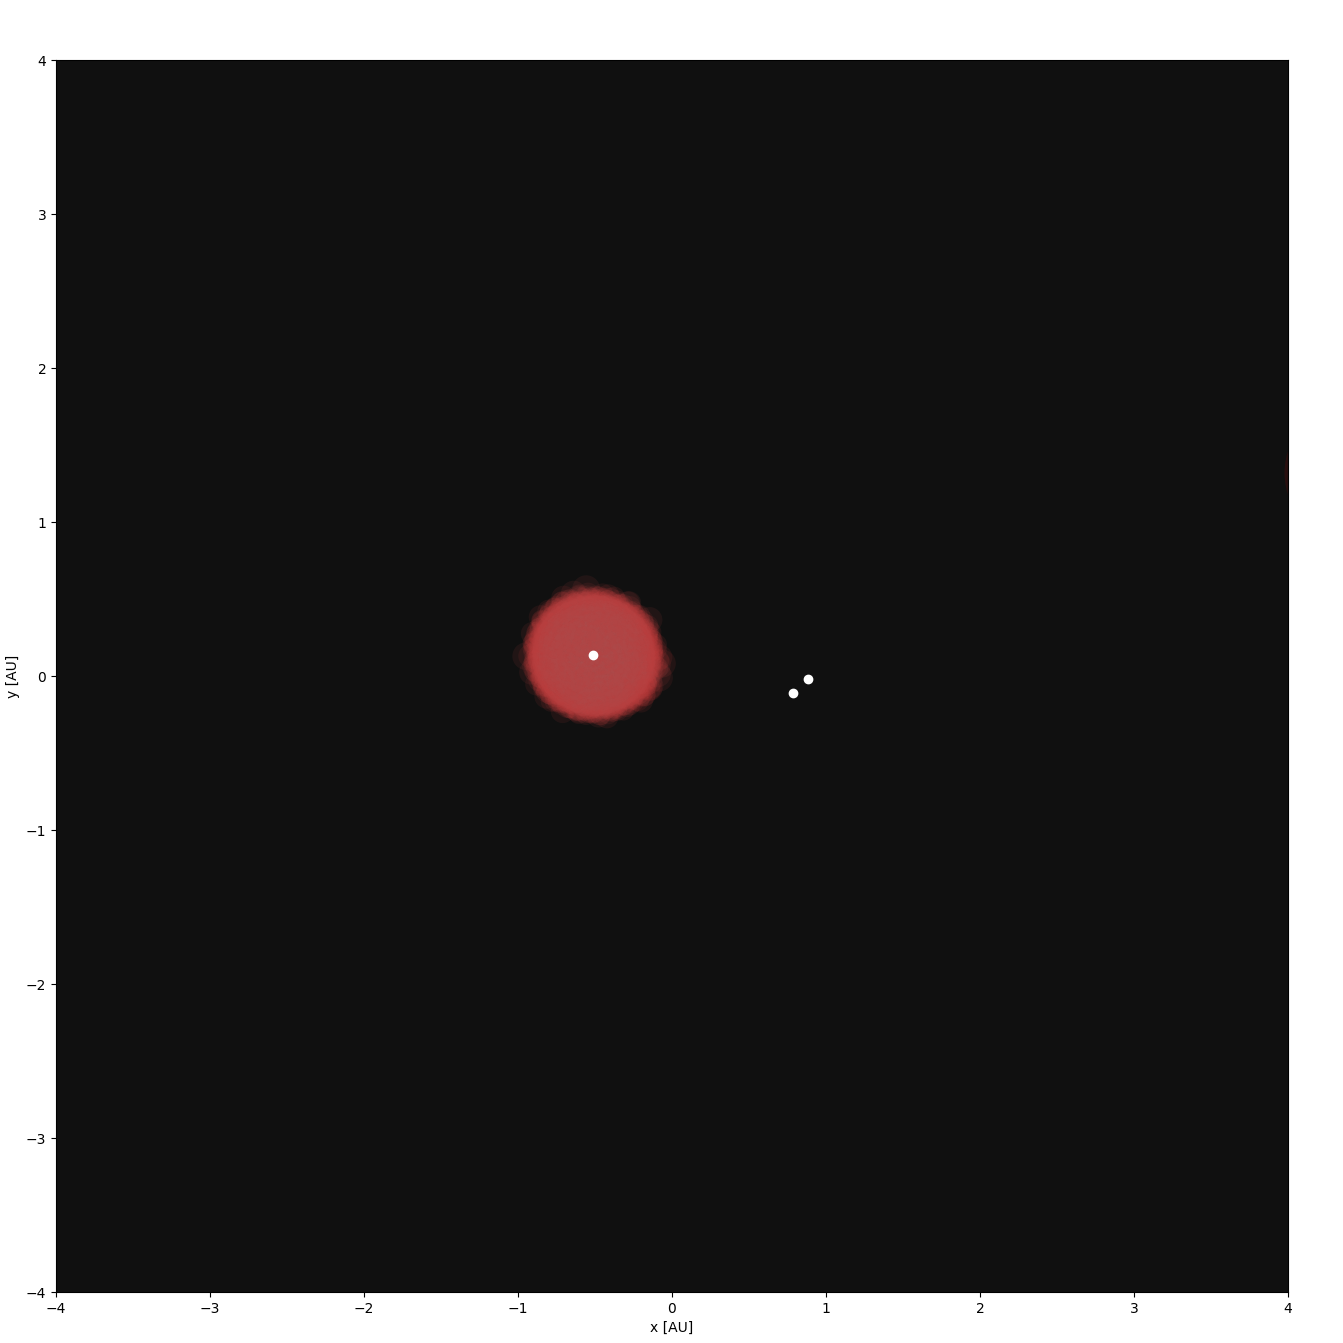
\includegraphics[width=\textwidth]{Thesis/graphs/hydro_triple_small0013687.png}   
    \end{subfigure}
    \hfill
    \begin{subfigure}[b]{0.49\textwidth}  
        \centering 
        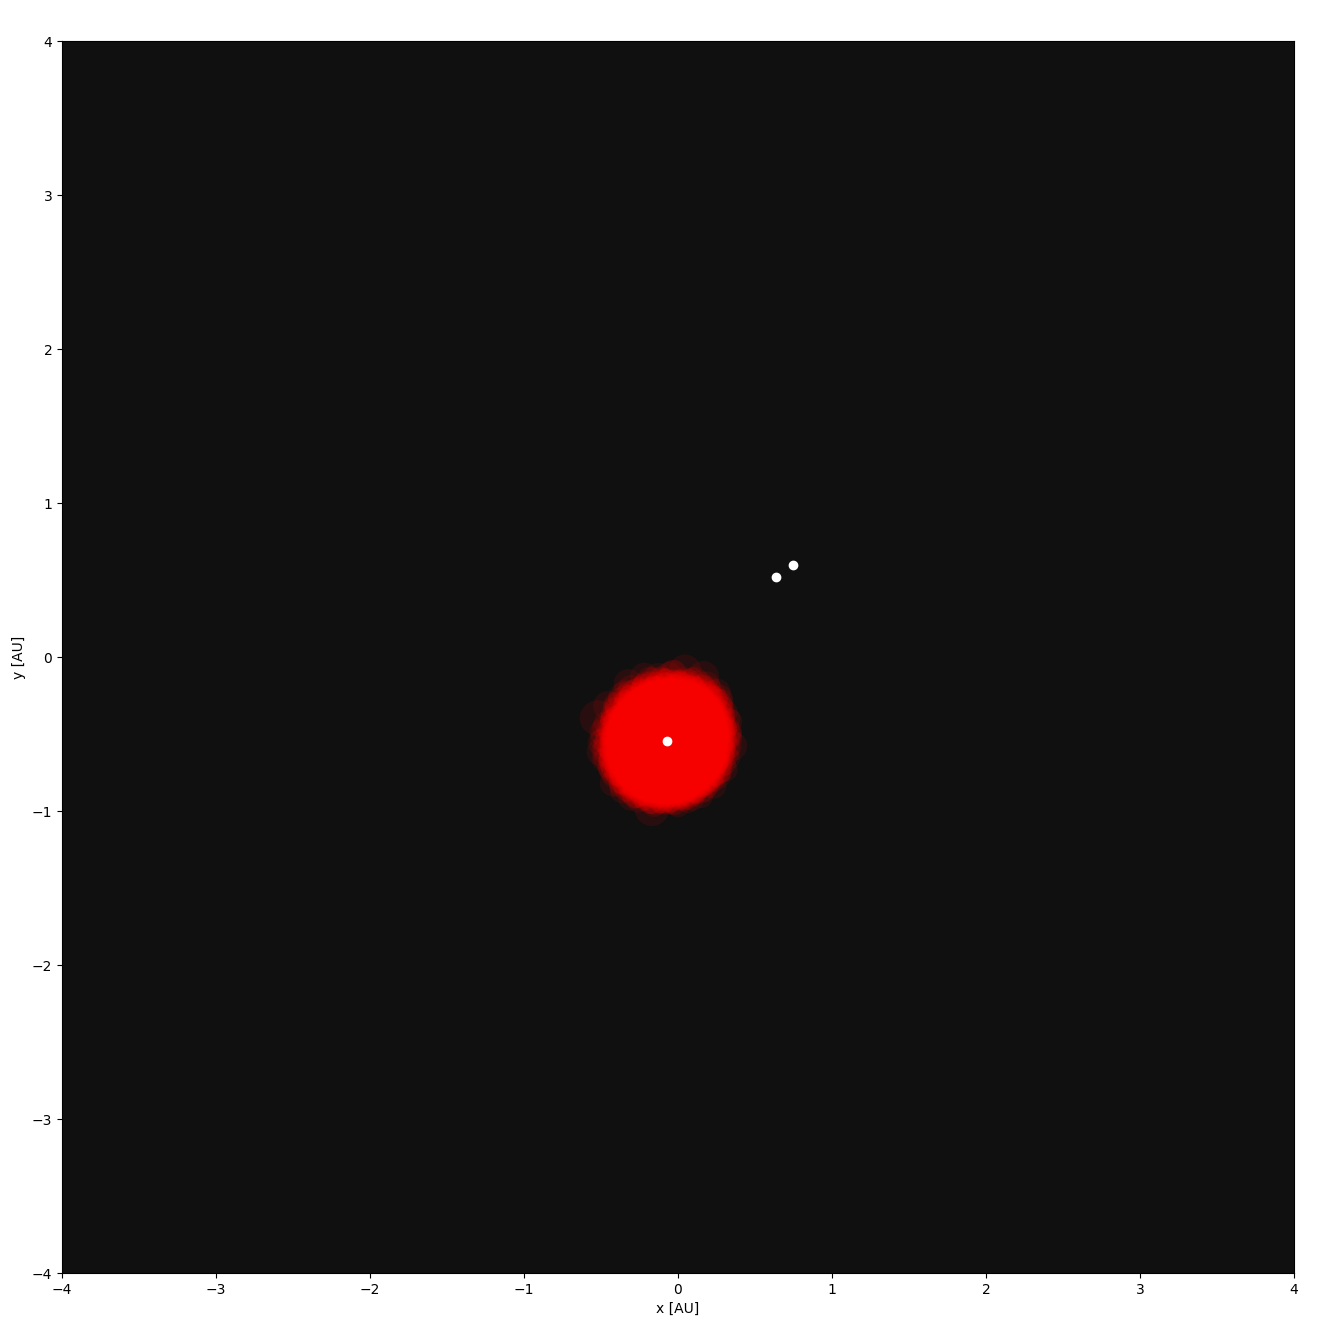
\includegraphics[width=\textwidth]{Thesis/graphs/hydro_triple_small0018250.png}
    \end{subfigure}
    \vskip\baselineskip
    \begin{subfigure}[b]{0.49\textwidth}  
        \centering 
        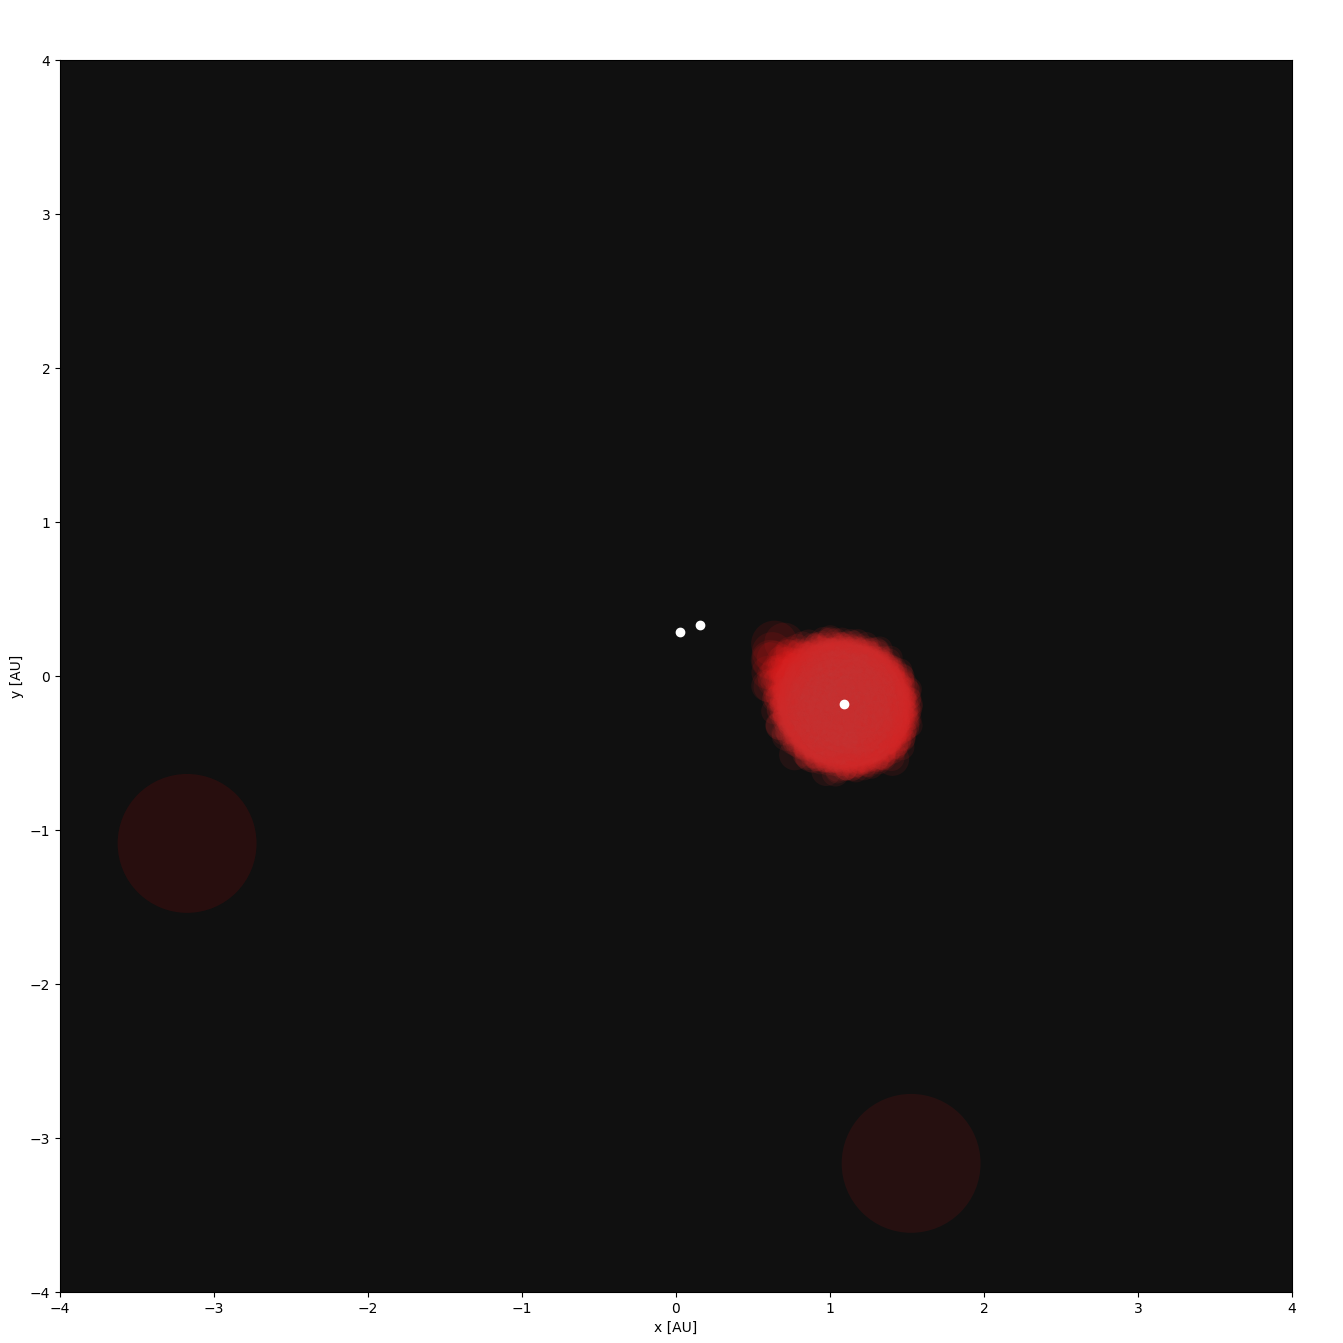
\includegraphics[width=\textwidth]{Thesis/graphs/hydro_triple_small0022812.png}
    \end{subfigure}
    \hfill
    \begin{subfigure}[b]{0.49\textwidth}  
        \centering 
        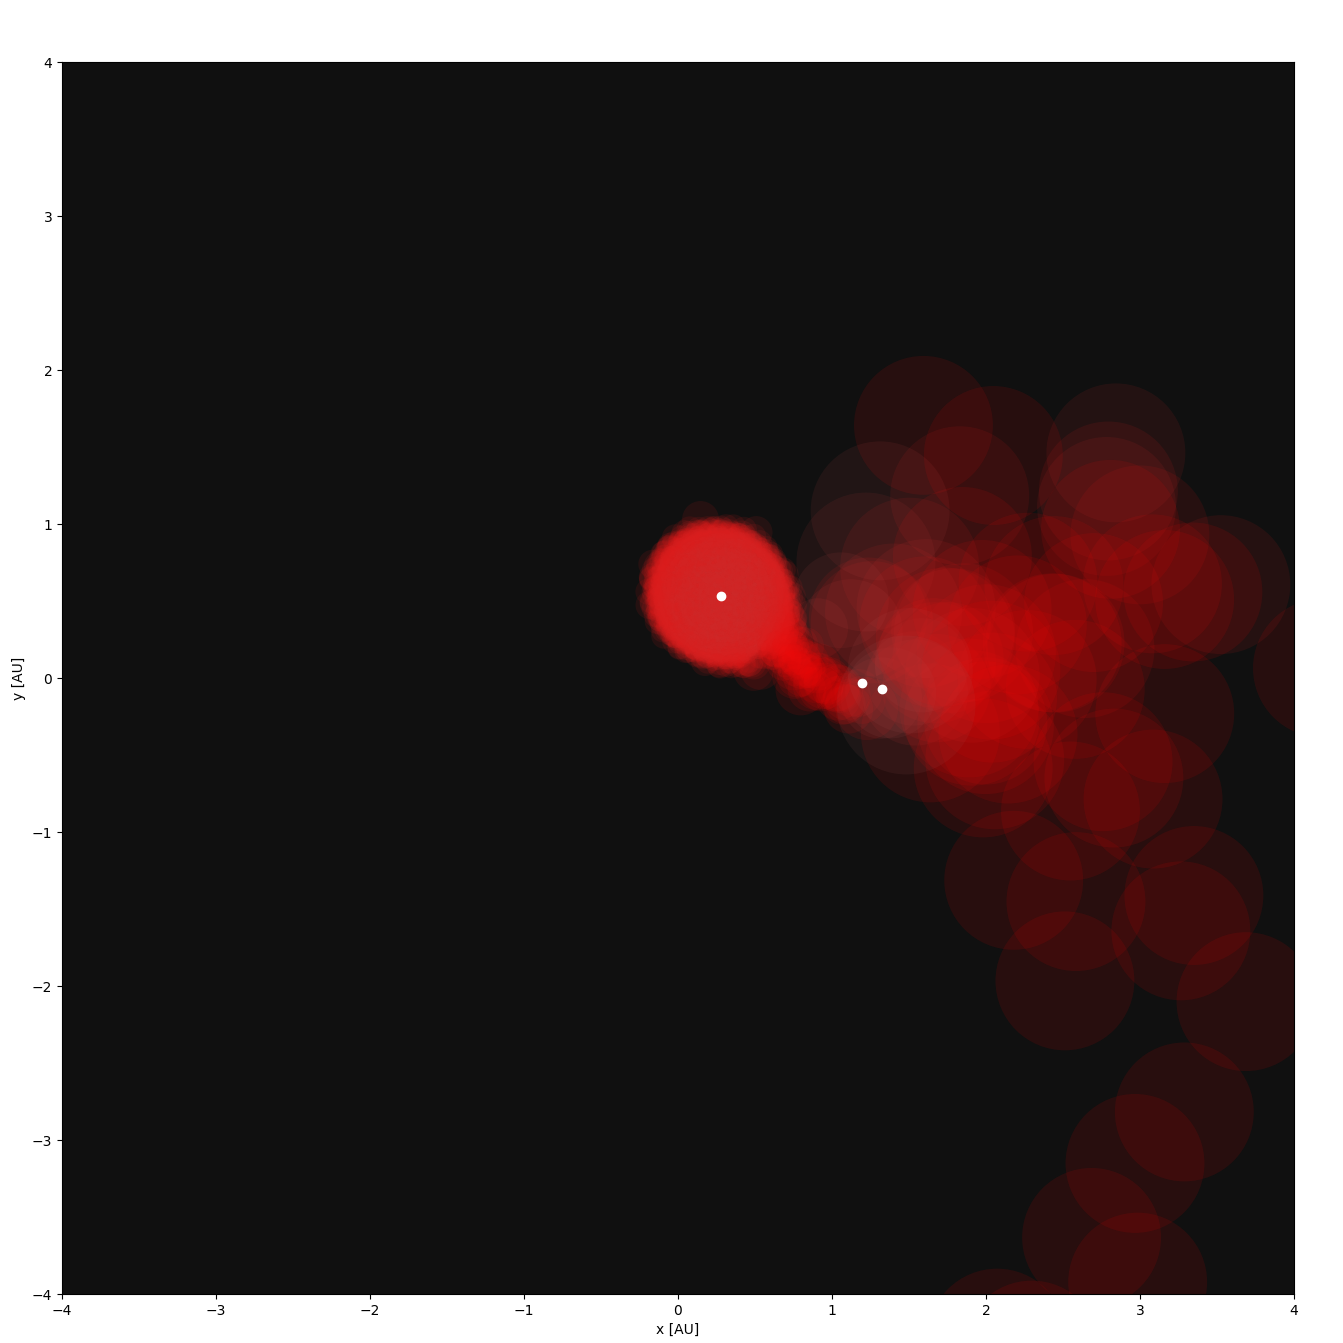
\includegraphics[width=\textwidth]{Thesis/graphs/hydro_triple_small0027375.png}
    \end{subfigure}
    \caption{System snapshots, from top to bottom and left to right, at 3.75, 5, 6.25 and 7.5 yr}
    \label{fig:simualtion_snapshots}
\end{figure}
Significant mass transfer from the tertiary towards the inner binary begins at $t \approx 4$ yr, so the time period of interest for my work begins at that point. The mass loss from the outer giant is periodic, modified by the outer orbit's periodicity, see \cref{fig:accretion_inc_00_mass_loss}. This is due to the slightly eccentric outer orbit, which causes the giant to overfill its Roche lobe at pericentre, but after semilatus rectum, the star detaches from its Roche lobe, to re-establish RLOF when it reaches pericentre again. As a result, the aforementioned periodicity is intrinsically carried through the evolution of the tertiary's mass too, see \cref{fig:accretion_inc_00_mass_loss}. Additionally, there is a significant delay between the moments of pericentre crossing and the maxima in mass transfer, see \cref{fig:simualtion_snapshots}, which is consistent with a study of RLOF in eccentric binaries \citep{lajoie2010mass}.
\begin{figure}[!htb]
    \centering
    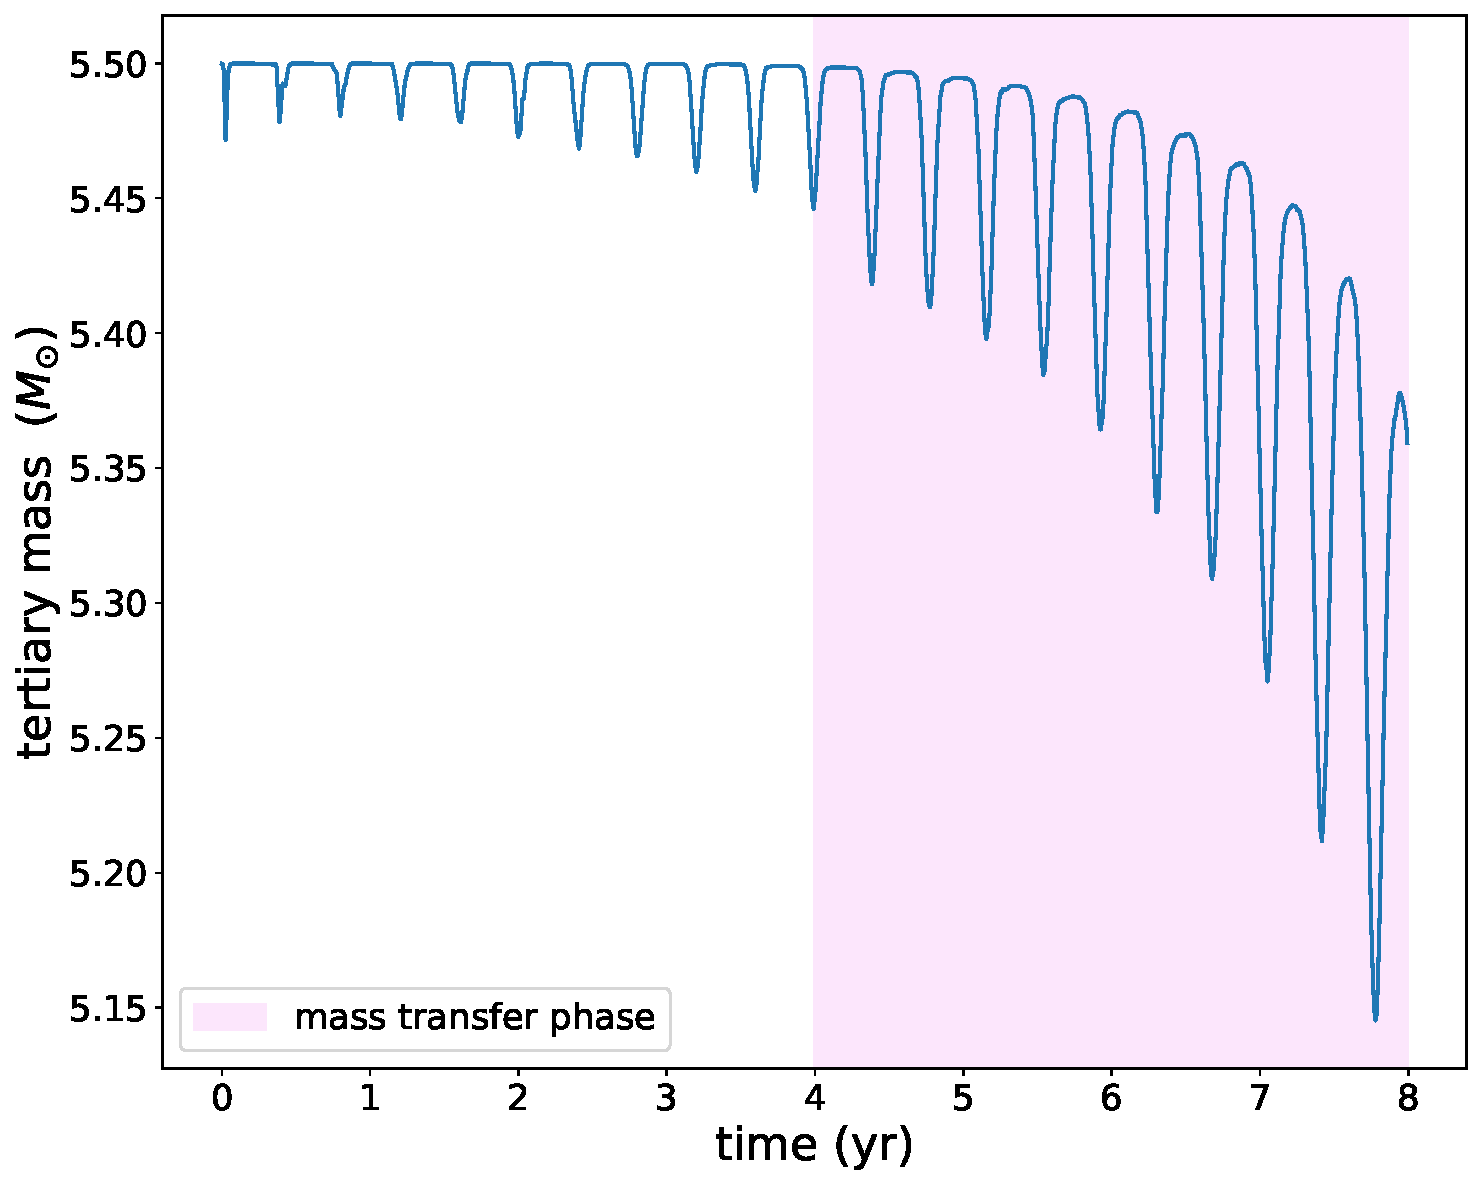
\includegraphics[width=0.85\textwidth]{Thesis/graphs/inc_00/accretion_inc_00_mass_loss.pdf}
    \caption{The evolution of the tertiary's mass.}
    \label{fig:accretion_inc_00_mass_loss}
\end{figure}
The mass transfer becomes progressively unstable, as expected for a donor with a convective envelope. Furthermore, the mass flowing from the first Lagrangian point of the outer orbit to the inner binary system interacts with the paths of the binary components. As a result, instead of a circumbinary disk, a gaseous cloud, similar to a common envelope (CE) \citep{ivanova2013common}, develops around the binary, see \cref{fig:simualtion_snapshots}. Part of the mass is being accreted by the inner binary and the rest escapes the system through the third Lagrangian point of the outer orbit, see \cref{fig:simualtion_snapshots}.

After eight years, which corresponds to $\approx 20$ orbits of the tertiary, the system enters the unstable regime, see \cref{eq:stability_regime}, and thus I terminate the simulations. Every $\delta t_{bridge}=0.1$ day, see \cref{tab:codes_settings}, I extract the mass, position and velocity of each particle in the computational domain. These properties are used to calculate the orbital parameters of the inner and the outer orbits. More specifically, the semi-major axis and eccentricity of the inner orbit are calculated using the relative position and velocity of the inner binary components. Furthermore, the relative position and velocity of the inner binary center of mass and the tertiary are used to determine the semi-major axis and eccentricity of the outer orbit. The calculations are based on \cref{eq:semi-major_axis} and \cref{eq:eccentricity}, where $M = M_1 + M_2$ and $M = M_1 + M_2 + M_3$ for orbital parameters of the inner and outer orbit, respectively. Finally, I calculate the outer orbit's relative inclination with respect to the inner orbit, i.e. mutual inclination, as the angle between their respective orbital angular momentum the vectors.

Despite being out of the scope of this work, it is worth noticing, that shortly after $t=8$ yr, the mass transfer becomes extremely unstable and a triple common envelope is encountered in all cases except for model number 3 listed in \cref{tab:simulations_settings}. For the rest models, the remainder of the tertiary's envelope engulfs the inner binary and the tertiary's core. In the case of $i_{mut} = 20^{\circ}$, the core of the tertiary is ejected from the system leaving behind a high eccentric binary. Finally, in both cases where the two orbits are initially coplanar, a direct collision completely disrupts the system.

\subsection{Outer orbit}

Tidal effects between the two orbits dominate the rates of change of orbital parameters up to $t \approx 4$ yr. The effect of mass transfer becomes visible after $t \approx 4$ years. A portion of the transferred mass is being accreted by the binary components, while the remainder is expelled from the system.  The ejected mass carries away orbital angular momentum, hence the outer orbit shrinks, see \cref{fig:accretion_inc_00_outer_semimajor_axis}. As a result,  the outer Roche lobe shrinks as well, see \cref{eq:roche_lobe}, and an increasing amount of mass can overflow towards the inner binary, see \cref{fig:accretion_inc_00_mass_loss}. 
\begin{figure}[H]
    \centering
    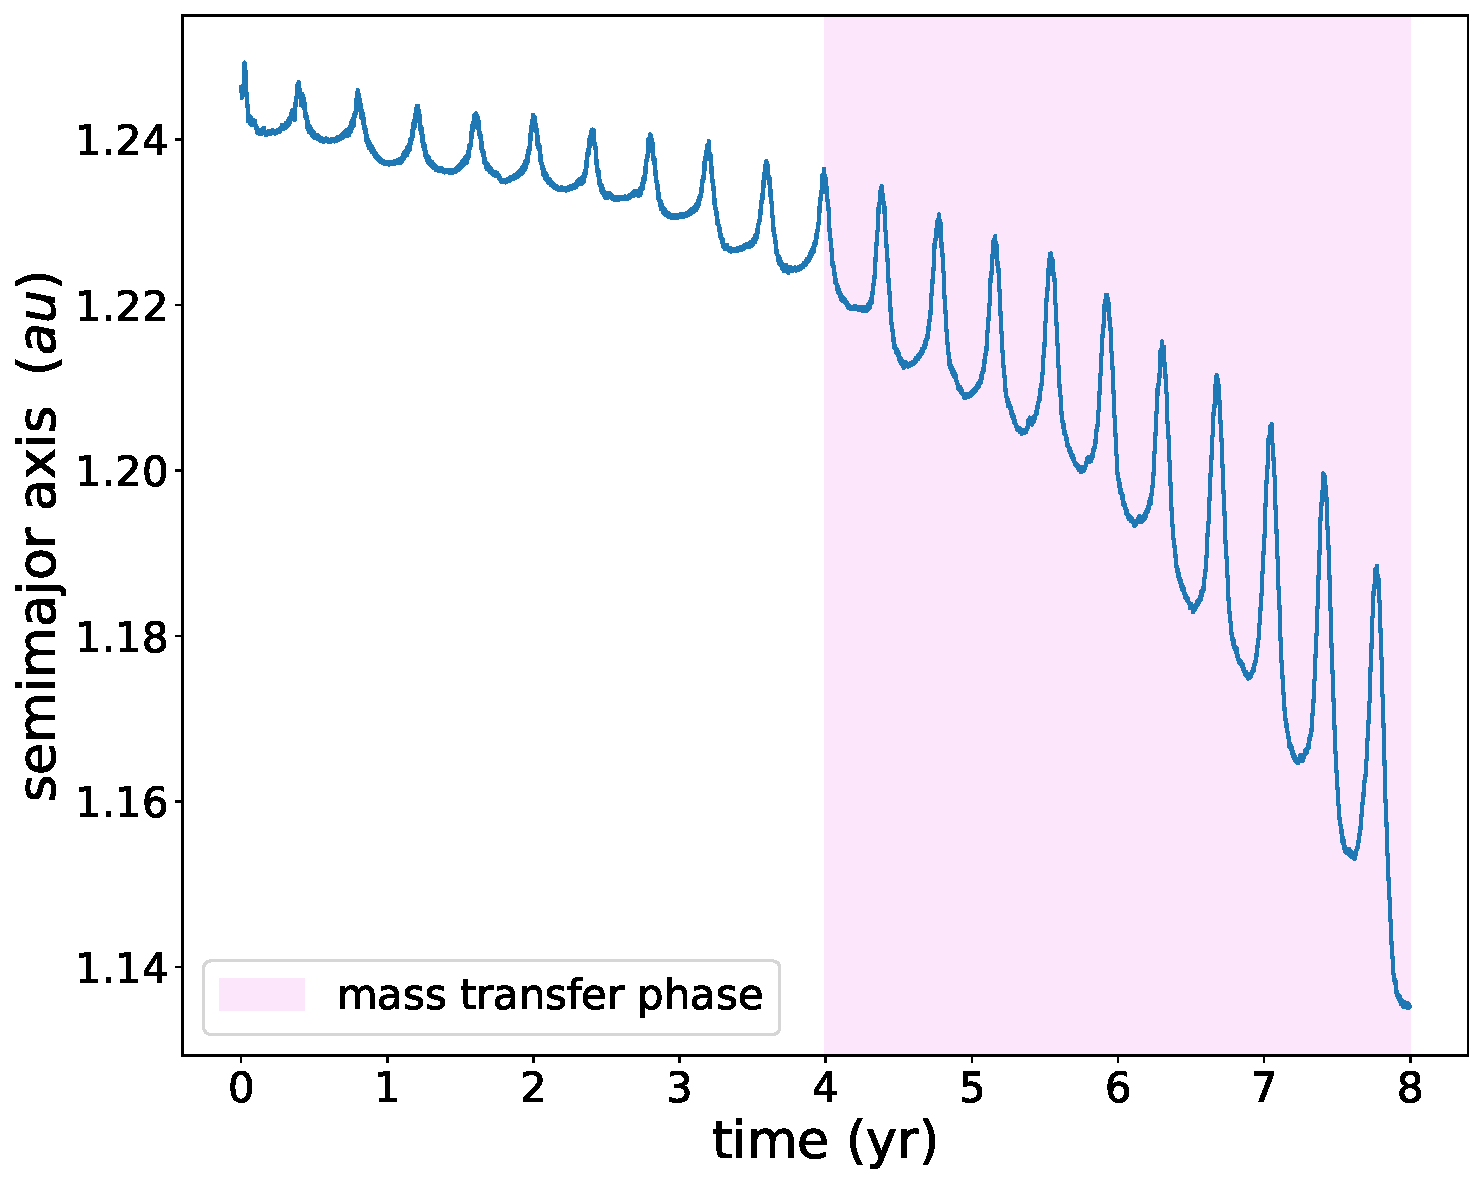
\includegraphics[width=0.85\textwidth]{Thesis/graphs/inc_00/accretion_outer_inc_00_semimajor_axis.pdf}
    \caption{Evolution of the semi-major axis of the outer orbit.}
    \label{fig:accretion_inc_00_outer_semimajor_axis}
\end{figure}
\begin{figure}[H]
    \centering
    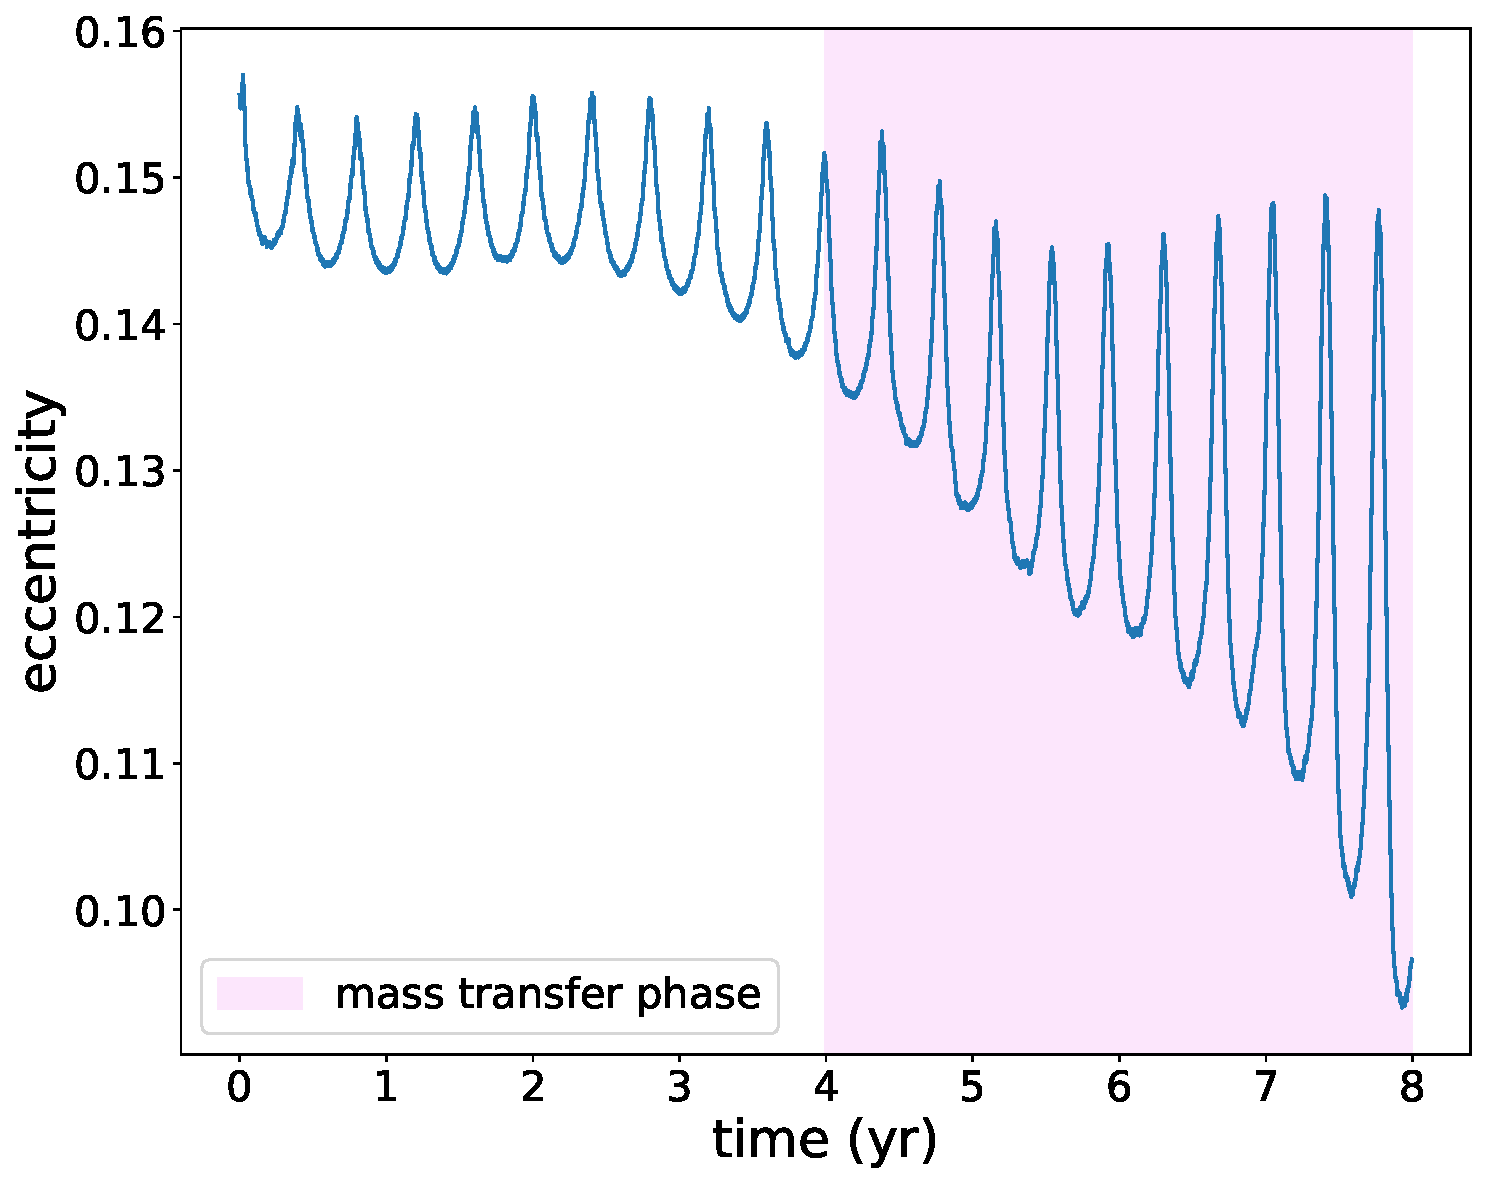
\includegraphics[width=0.8\textwidth]{Thesis/graphs/inc_00/accretion_inc_00_outer_ecc.pdf}
    \caption{Evolution of the eccentricity of the outer orbit.}
    \label{fig:accretion_inc_00_outer_ecc}
\end{figure}
\begin{figure}[H]
    \centering
    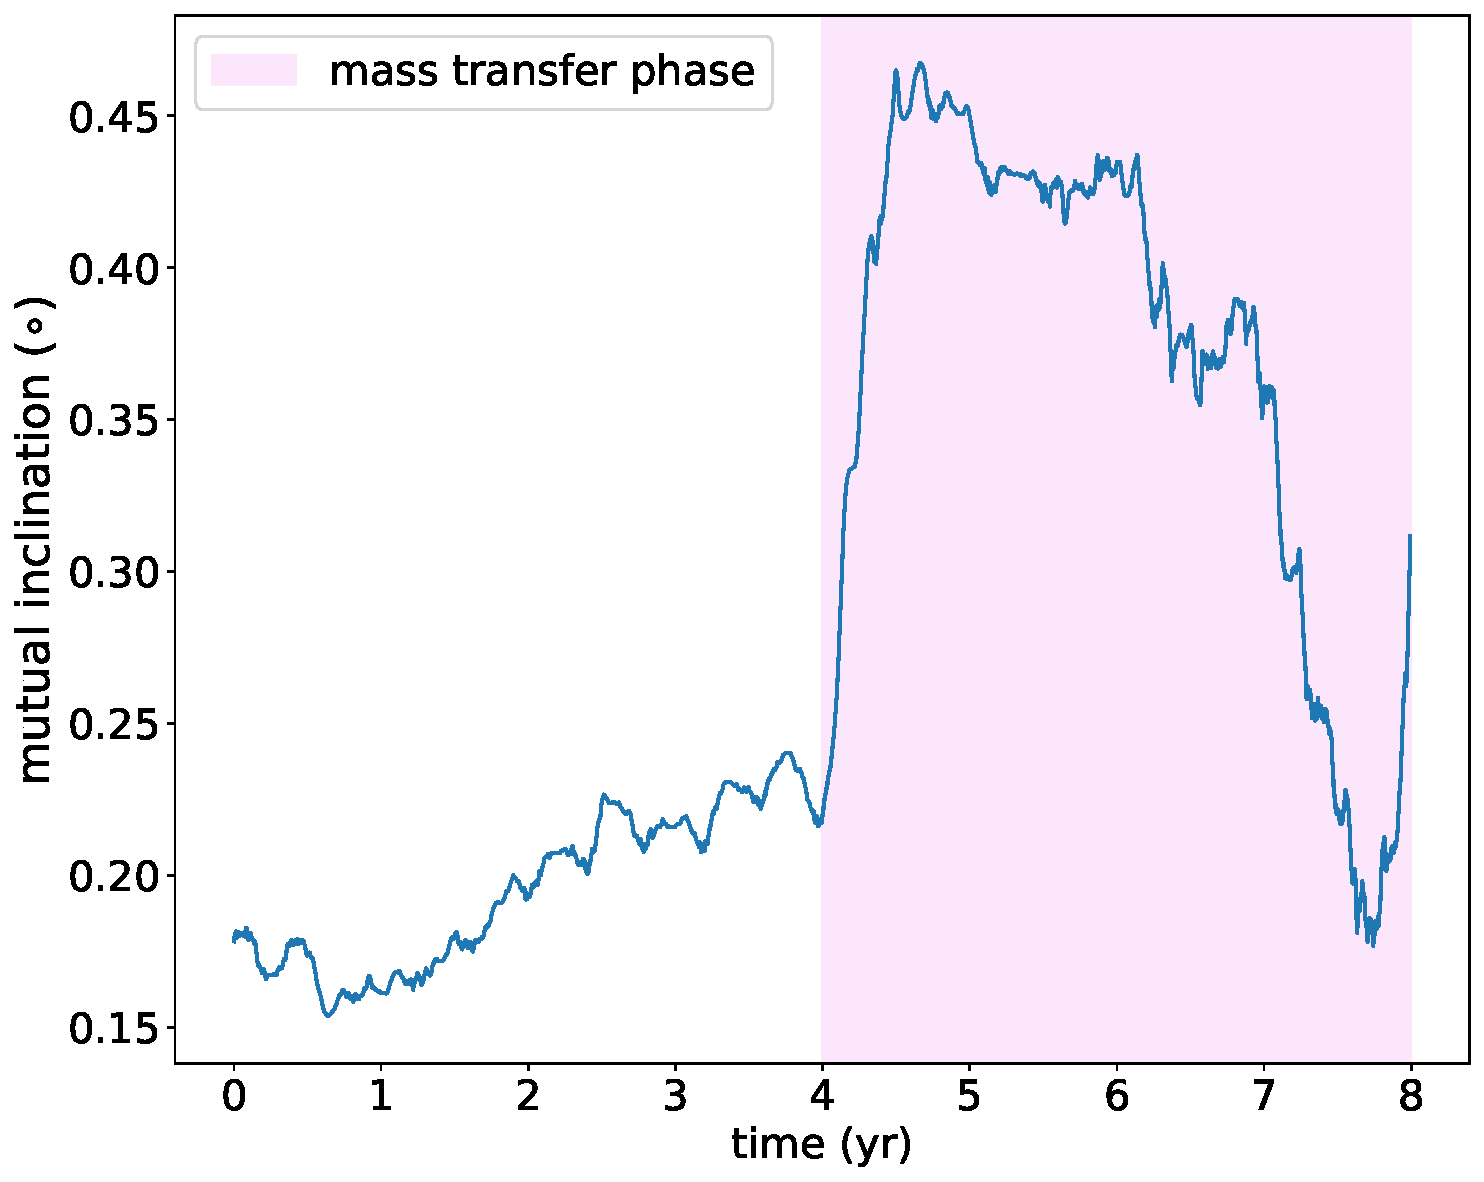
\includegraphics[width=0.8\textwidth]{Thesis/graphs/inc_00/accretion_inc_00_inc.pdf}
    \caption{Evolution of the inclination of the outer orbit relative to the inner orbit.}
    \label{fig:accretion_inc_00_inc}
\end{figure}
Furthermore, as the tertiary approaches the inner binary, tidal effects between the two orbits become stronger. Tides tend to circularize and flatten the outer orbit. \cref{fig:accretion_inc_00_outer_ecc} shows the former, while \cref{fig:accretion_inc_00_inc} shows the latter, where the outer orbit, which is already coplanar with the inner orbit, remains close to coplanarity.


\subsection{Inner orbit}

As the transferred mass intersects the inner orbit, the binary components interact with the gas. Some of the gas is being accreted, while some is ejected from the binary's close vicinity. The inner binary is generally influenced by hydrodynamics, notably gas drag, which always tends to shrink the orbit. Furthermore, by the accretion process and the inner orbit's gravitational interaction with the incoming material stream. The effect of the later on the evolution of the orbit is complex and depends on the angle at which the mass stream crosses the inner obit. This is discussed in more detail in \cref{sec:inclination}. 

In \cref{fig:accretion_inc_00_inner_semimajor_axis} and \cref{fig:accretion_inc_00_inner_ecc}, I present the evolution of the semi-major axis and eccentricity of the inner orbit, 
respectively. Both graphs show the presence of the tertiary, which introduces the observed fluctuations with periods equal to the period of the outer orbit, $\Delta t \approx 145.5$ days.
\begin{figure}[H]
    \centering
    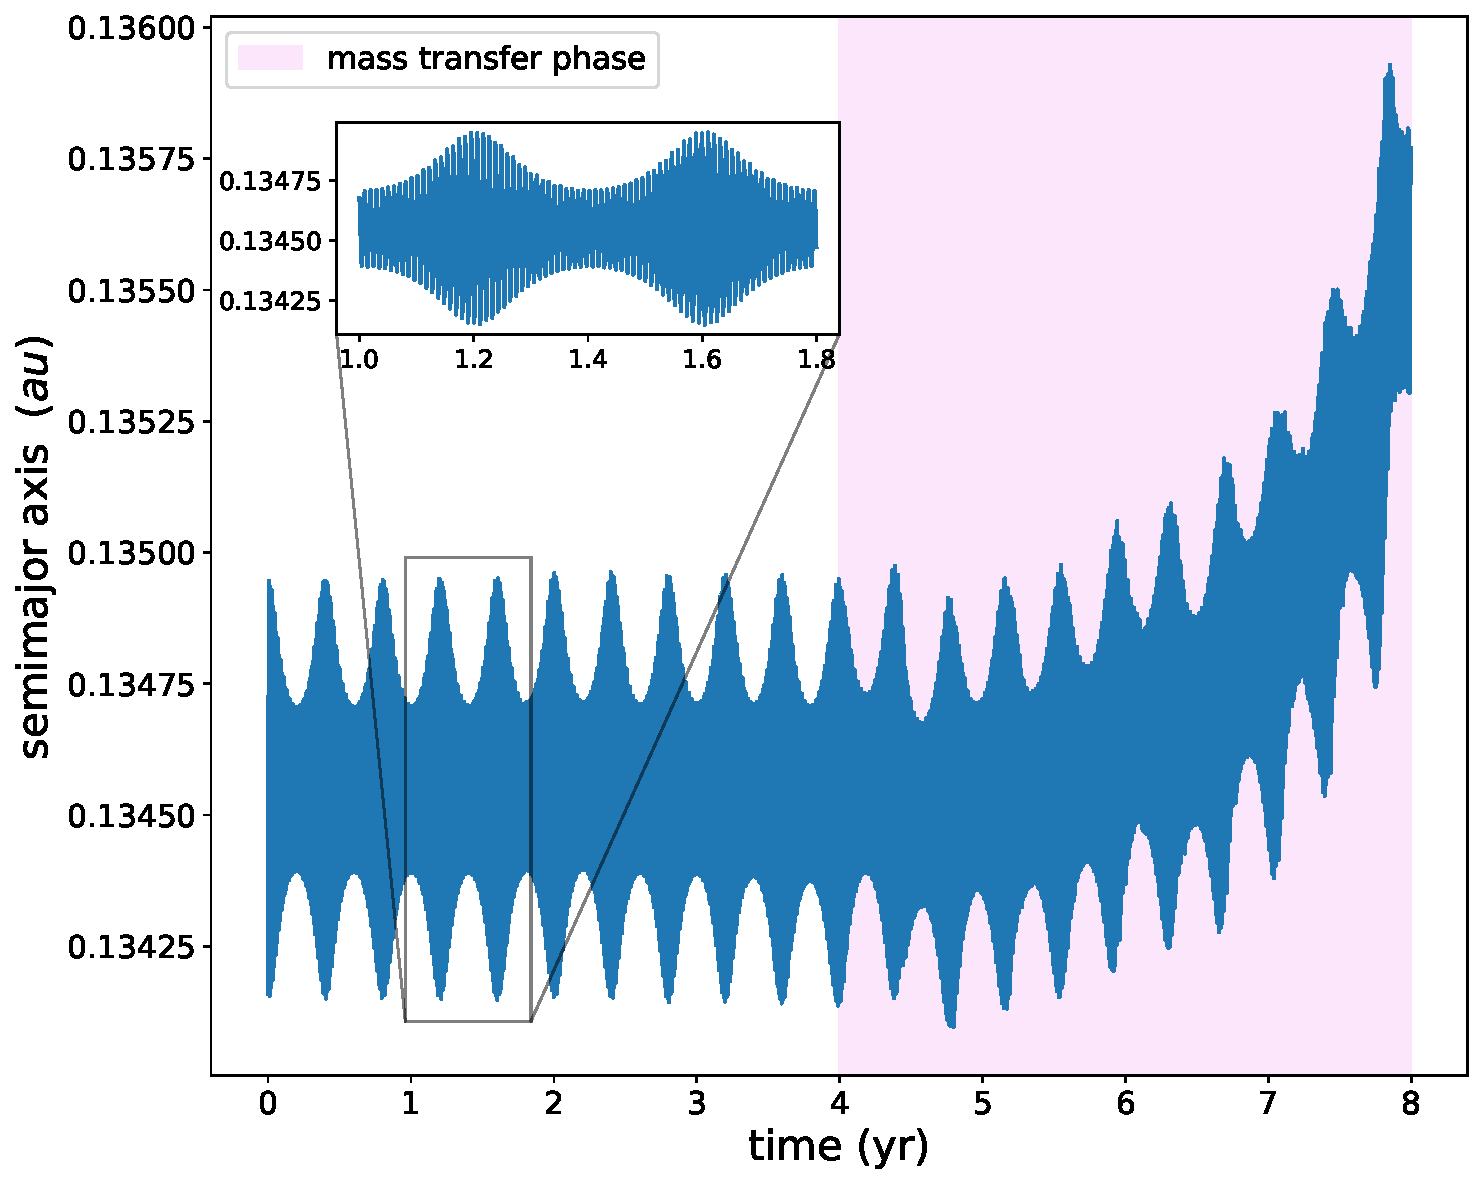
\includegraphics[width=0.9\textwidth]{Thesis/graphs/inc_00/accretion_inc_00_inner_semimajor_axis.pdf}
    \caption{Evolution of the semi-major axis of the inner orbit.}
    \label{fig:accretion_inc_00_inner_semimajor_axis}
\end{figure}
In the case where the inner and outer orbit are coplanar the former seems to widen, see \cref{fig:accretion_inc_00_inner_semimajor_axis}. 
This is an unexpected outcome, because a common envelope-like structure around the binary is encountered and a detailed discussion is taking place in \cref{sec:resolution}. Furthermore, the effect of mass transfer on the eccentricity of the inner orbit is negligible and the orbit remains circular. 
\begin{figure}[!htb]
    \centering
    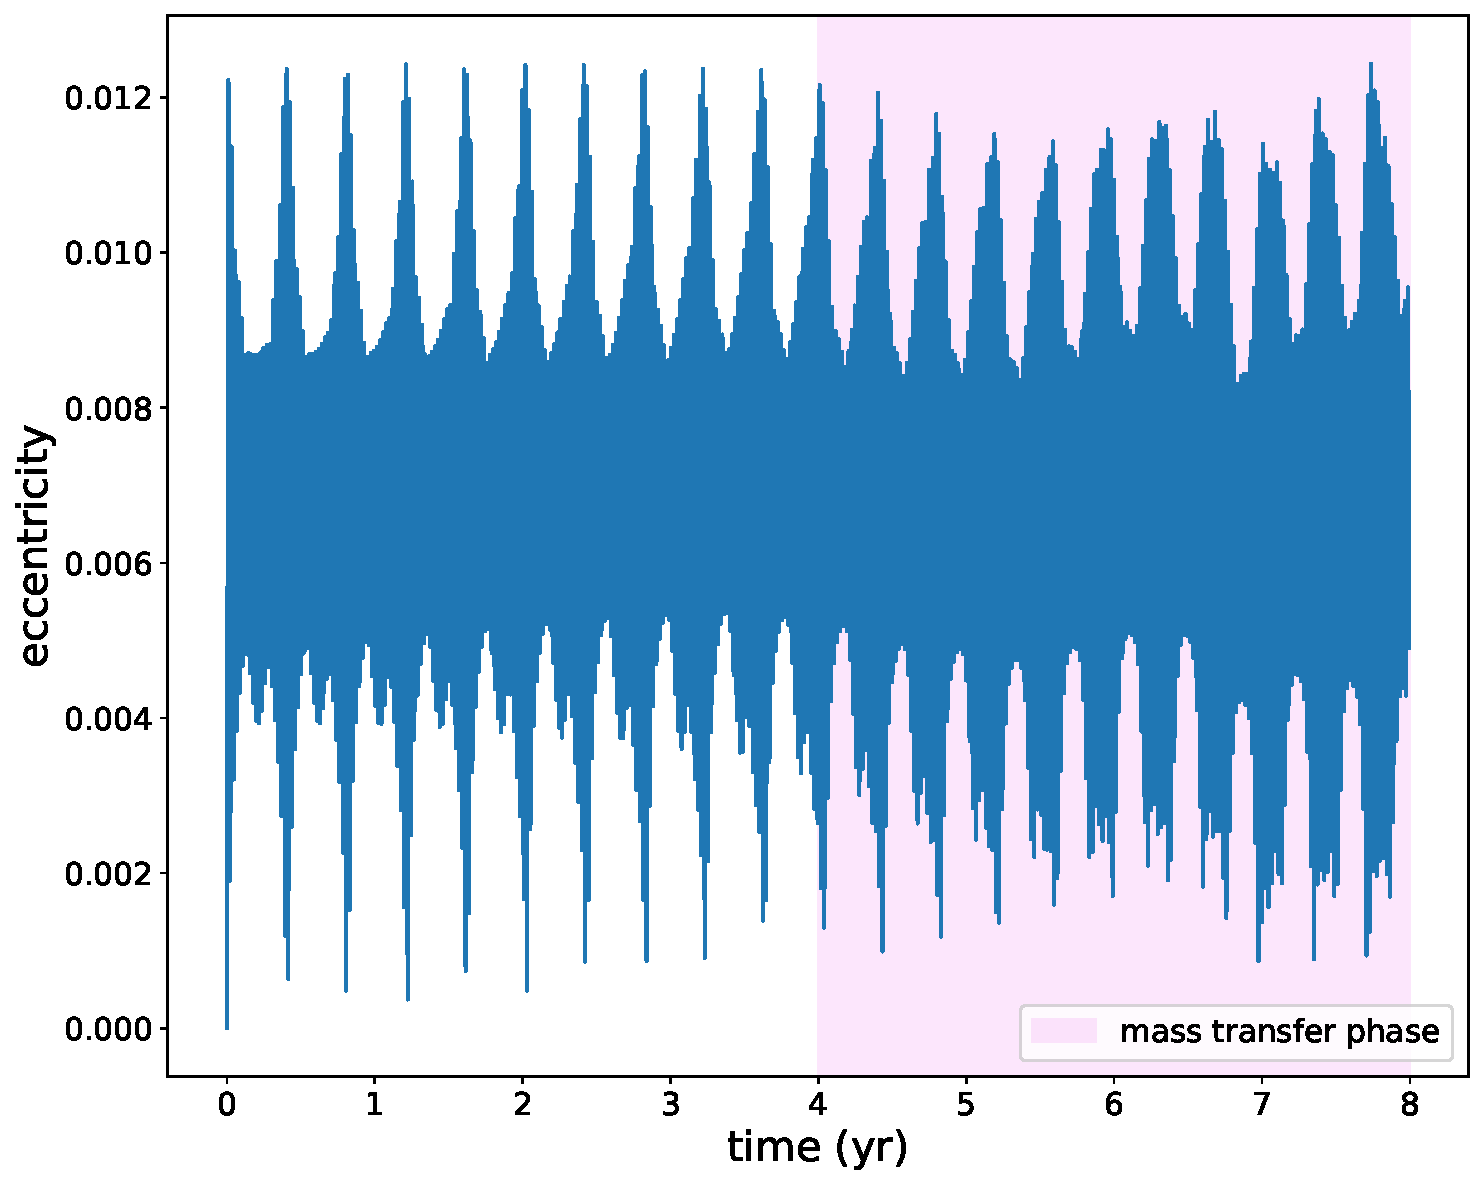
\includegraphics[width=0.9\textwidth]{Thesis/graphs/inc_00/accretion_inc_00_inner_ecc.pdf}
    \caption{Evolution of the eccentricity of the inner orbit.}
    \label{fig:accretion_inc_00_inner_ecc}
\end{figure}




\section{Resolution Benchmark}\label{sec:resolution}

In the general case of RLOF by an outer star towards an inner binary, the response of the latter's orbit may vary. \cite{zwart2019triple} investigate the case in which the incoming mass stream forms a circumbinary disk. They find that the details of the accretion can cause the inner orbit to shrink, a behavior that reverses though assuming a more massive donor. In the case where a common envelope-like structure is formed around the inner binary, the orbit is expected to shrink \citep{de2014evolution}. Given that the efficiency of the gas drag in shrinking the inner orbit must be strongly related to the density of the gas cloud surrounding the inner binary, I need to investigate whether the observed behavior, see \cref{fig:accretion_inc_00_inner_semimajor_axis}, is a physical result or the result of poor resolution (small number of SPH particles).

The smoothing length is determined by the number of SPH particles in a region of the computational domain, which in turn defines the simulation's resolution in that region, see \cref{sub:gadget2}. The latter is small in high-density regions and large in low-density regions. To correctly account for the influence of gas drag on the inner binary, the smoothing length of the particles interacting with it must be considerably smaller than the binary's size. In my simulations, $N=50000$ is used. 

A simulation's snapshot at $t \approx 7.5$ yr is illustrated in \cref{fig:resolution}, where the mass transfer is maximum. The x-axis represents the distance of each particle from the tertiary's center of mass, while the y-axis represents the smoothing length of each particle. The horizontal yellow line corresponds to the orbital separation of the inner binary components, i.e. the binary's size. Finally, the red area represents an approximation of the inner binary's close vicinity. More specifically, it corresponds to the position of the inner binary's center of mass $\pm$ the binary's size.
\begin{figure}[!htb]
    \centering
    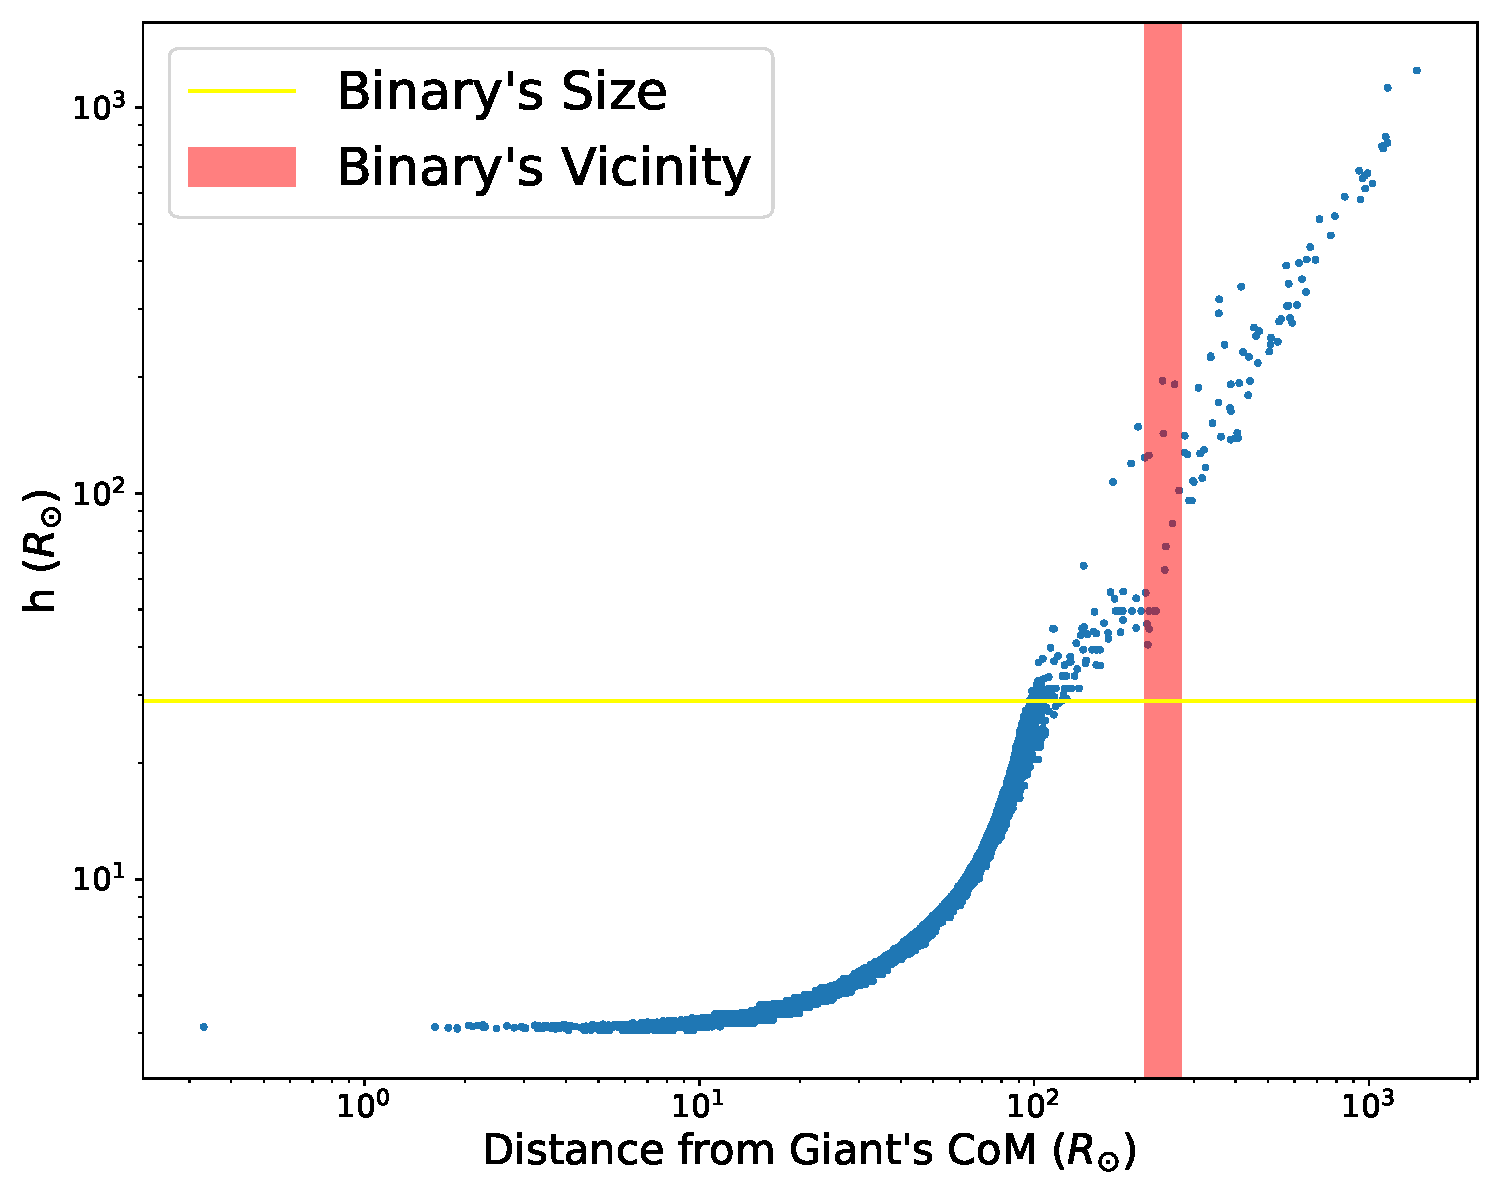
\includegraphics[width=0.9\textwidth]{Thesis/graphs/resolution_benchmark.pdf}
    \caption{Particles smoothing lengths in comparison to the binary's size at $t \approx 7.5$ yr, where the mass transfer is maximum.}
    \label{fig:resolution}
\end{figure}

Particles with smoothing lengths smaller than the binary's size, blue points bellow the yellow line, and close to the binary, blue points close/inside the red region, can influence hydrodynamically the inner orbit. At the current resolution, even when the mass transfer is maximum, the number of particles interacting with the binary is small (low-density mass stream), and thus their smoothing length is much larger than the size of the inner orbit, hence the present resolution probably underestimates the effect of gas drag. In conclusion, higher resolution simulations are required to safely estimate the evolution of the semi-major axis of the inner orbit.

Given the underestimation of gas drag and the resulting development depicted in \cref{fig:accretion_inc_00_inner_semimajor_axis}, I ran a test simulation in which the initial inner and outer orbital angular momentum vectors are antiparallel. In the parallel case, see orange line in \cref{fig:retro}, accretion and gravitational interactions between the stars and the incoming mass stream appears to work as a slingshot effect in favor of the stars. Whereas in the antiparalel scenario, it appears to act as a braking mechanism for the stars, see blue line in \cref{fig:retro}. The reason behind this behavior is the following: When a sink accretes a gas particle, its mass and momentum are added to the star. Because momentum is a vector, the acceleration or deceleration of the star must be determined by the relative vector of the star's and the particle's velocity. This implication explains the observed trend in \cref{fig:accretion_inc_00_inner_semimajor_axis} and it is further investigated in \cref{sec:inclination}.
\begin{figure}[!htb]
    \centering
    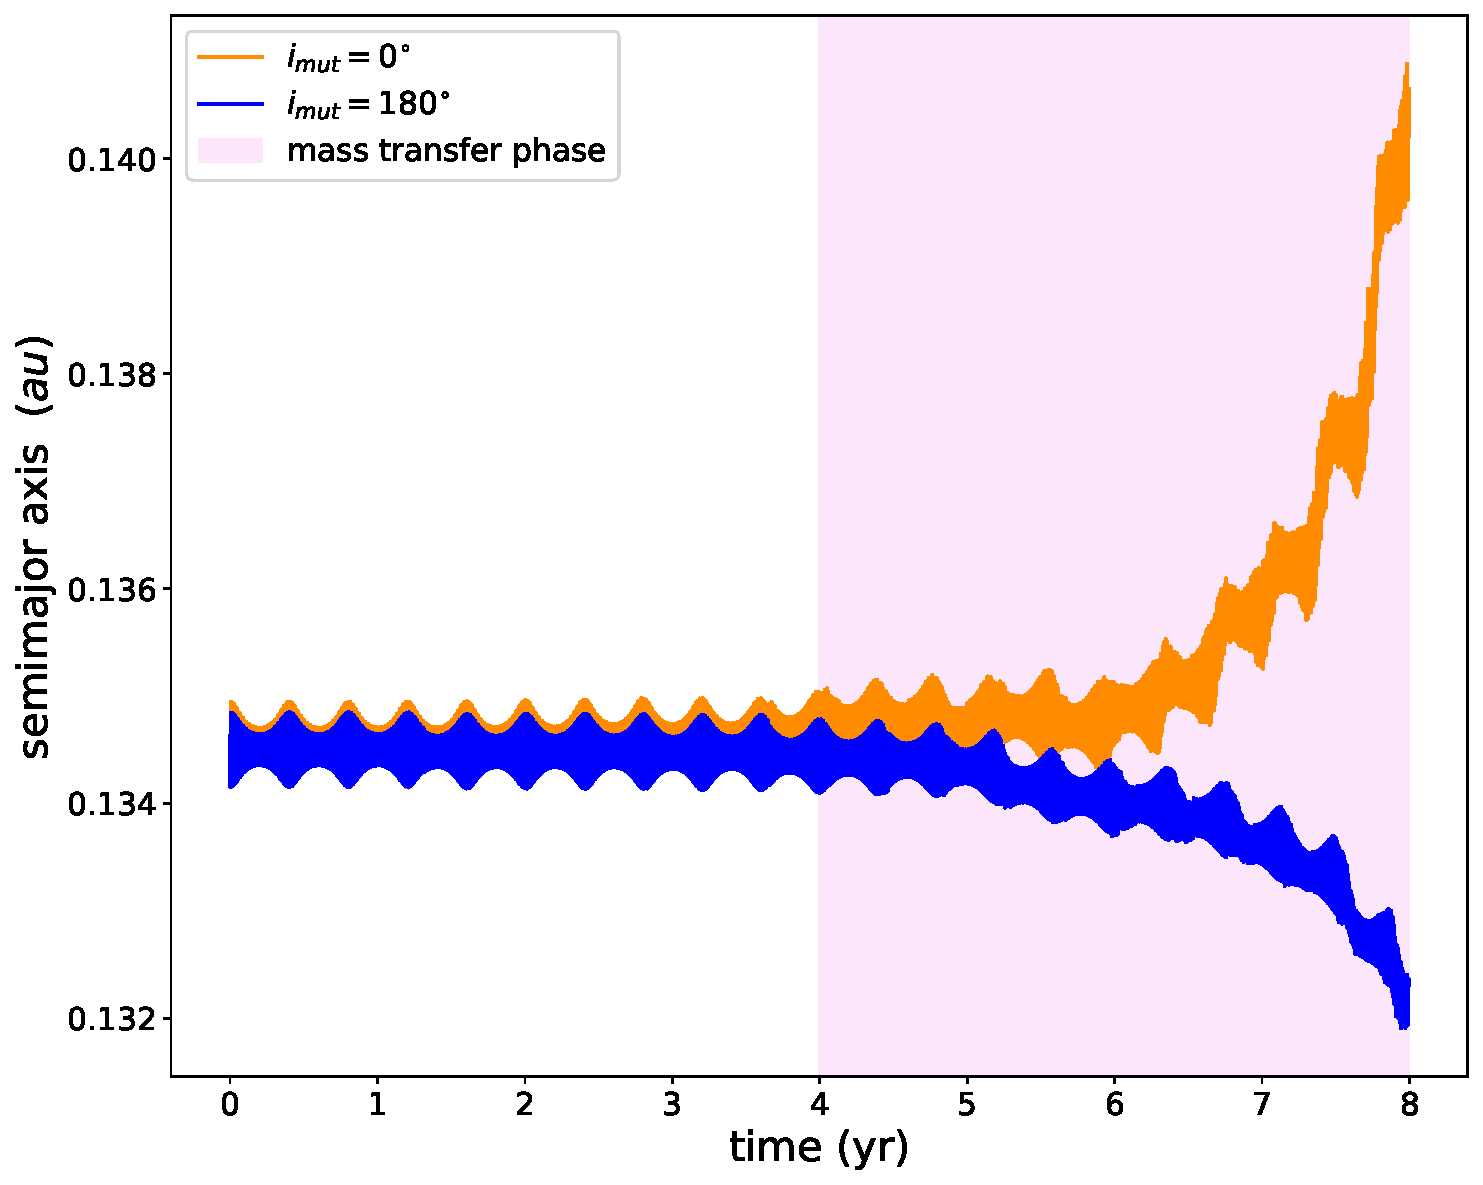
\includegraphics[width=0.9\textwidth]{Thesis/graphs/accretion_inc_00_retro_inner_semimajor_axis.pdf}
    \caption{Evolution of the semi-major axis of the inner orbit. The orbital angular momentum of the inner and outer orbit are parallel and antiparallel for the the orange and blue lines, respectively.}
    \label{fig:retro}
\end{figure}

Despite the fact that $N=50000$ is sufficient to initially resolve the giant at the moment of RLOF, see \cref{sec:1D_to_3D}, it is insufficient to accurately capture the gas drag on to the inner orbit. The fact that \cite{de2014evolution} use also $N=50000$ to examine mass transfer via RLOF by the outer star, for the same system was a motivation behind this particular choice. In their study, they employ a different SPH code. Nevertheless, both codes define the particles smoothing length in a similar fashion, thus it is a surprise that they are able to account for gas drag at seemingly the same resolution. 

To achieve higher resolution, I could simply increase the number of particles in my simulation. This is pretty straight forward in my code, however time restrictions require me to consider leaving this for future work. More specifically, with the available computational resources I obtain eight years of simulation in approximately five weeks of computational run time. Considering that the CPU time scales with the number of \ac{sph} particles as $NlogN$, increasing the number of particles by a factor of 5 results in several months of computational run time. 

In conclusion, with the current number of \ac{sph} particles the resolution of my simulations is probably insufficient to accurately capture the influence of the gas drag on the inner orbit. As a result, the gas drag is underestimated, while the models capture the gravitational interactions between the inner binary, the core of the tertiary, and its gaseous envelope. Regardless, I can still extract useful information about the evolution of the outer orbit and conjecture about the evolution of the inner orbit. 

\section{Impact of accretion}\label{sec:accretion}

In this section, I compare models  1 \& 4 listed in \cref{tab:simulations_settings}, which correspond to the maximum and minimum accretion case, respectively. Here, I examine the effects of accretion on the evolution of the system.

In \cref{sec:mass_transfer_RLOF}, I showed that periodic variations are naturally integrated in my models due to the outer orbit's eccentricity. The key point though, is that the timescale of this periodicity is equal to the period of the outer orbit. In the parent and next section, I focus on the global evolution of the orbital parameters. As a result, the presented graphs associated with the outer orbit, display not only the original output of my simulations, but also smoothed versions of it. A kernel of width equal to $3 \times P_{out}$ is used to smooth the data. The is for illustration purposes only, as it is easier for the reader to follow the comparison between the models listed in \cref{tab:simulations_settings}. 

\subsection{Outer orbit}

In \cref{fig:accretion_outer_semimajor_axis}, \cref{fig:accretion_outer_ecc} and \cref{fig:accretion_inc}, I display the evolution of the semi-major axis, eccentricity and the inclination of the outer orbit relative to the inner orbit, respectively.

For the minimum accretion case, the outer orbit decays faster, see \cref{fig:accretion_outer_semimajor_axis}. This behavior is expected, because more mass is lost from the system and the ejected mass carries away orbital angular momentum. Furthermore, as the tertiary approaches the inner binary, tidal effects between the two orbits become stronger. Tides tend to circularize and flatten the outer orbit. More specifically, in the equilibrium-tide model, the circularization timescale is $\propto \frac{R_{\star}}{\alpha}^{-8}$ and the faster decay of the orbit leads to a faster circularization too, see \cref{fig:accretion_outer_ecc}. Finally, in both cases, the outer orbit, which is already coplanar with the inner orbit, remains close to coplanarity, see \cref{fig:accretion_inc}.
\begin{figure}[H]
    \centering
    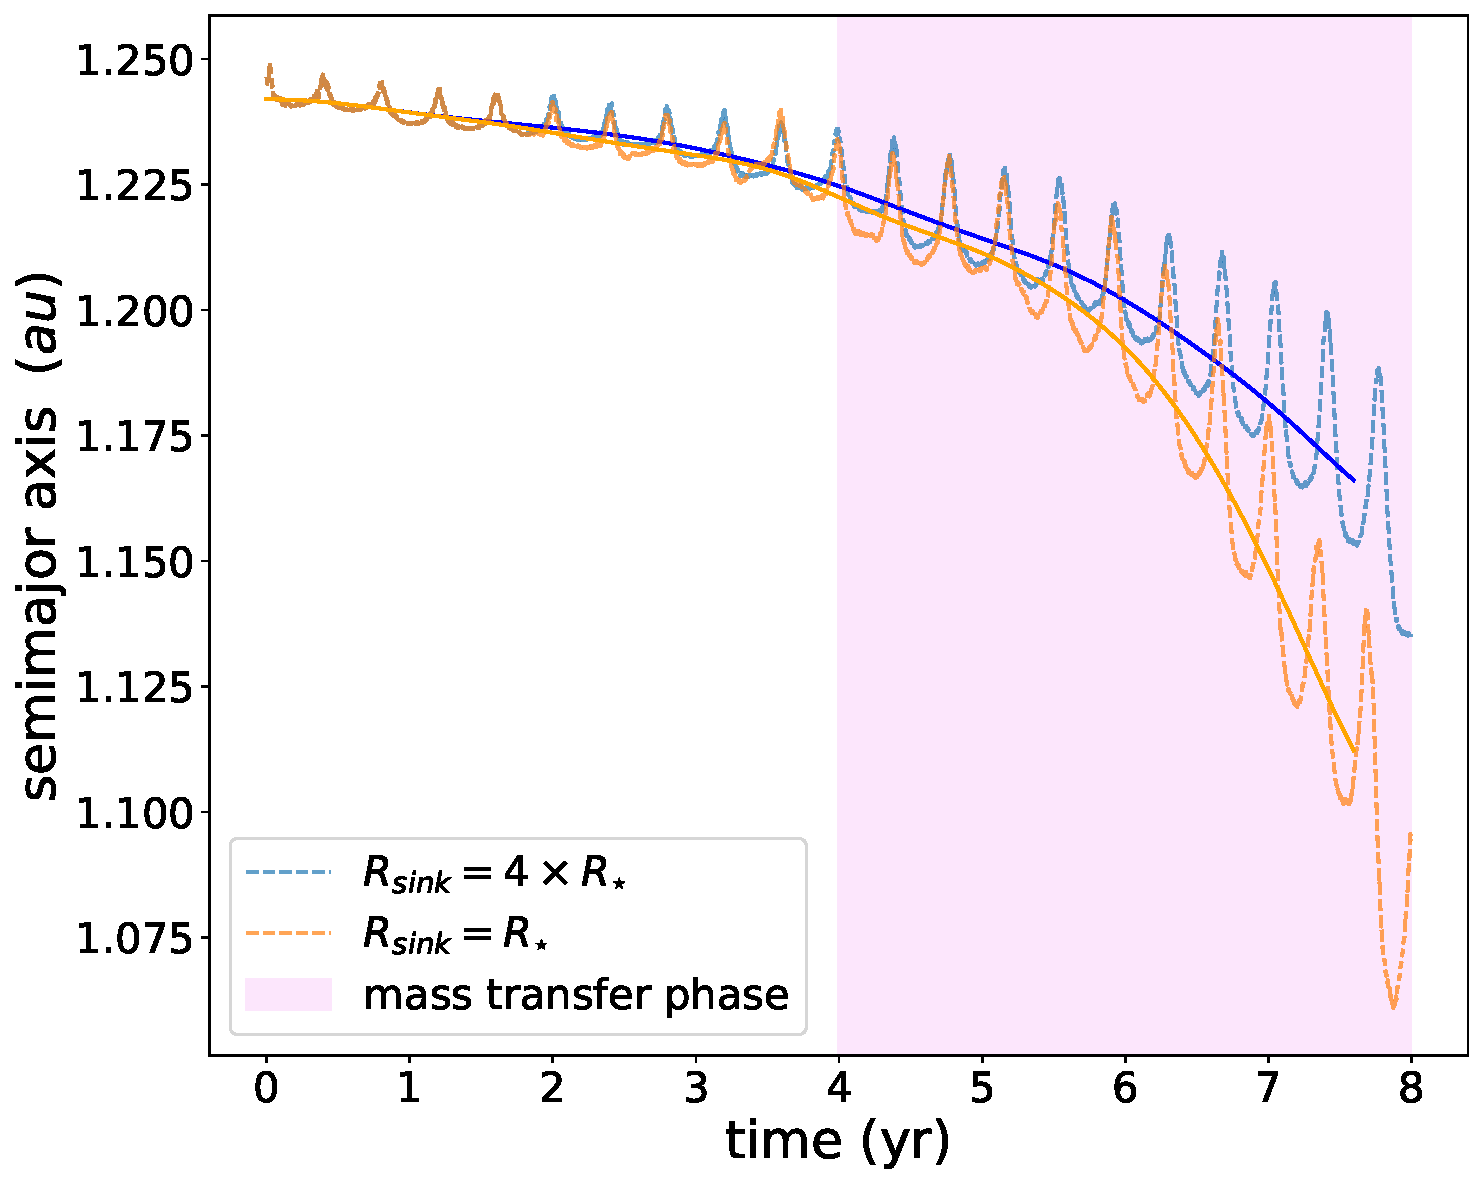
\includegraphics[width=0.9\textwidth]{Thesis/graphs/accretion_case/accretion_outer_semimajor_axis.pdf}
    \caption{Evolution of the semi-major axis of the outer orbit for the minimum and maximum accretion case. The simulated data is shown in dashed lines. The continues lines are smooth representations of the simulated data in their respective colors. The last three orbits are not included in the smoothed version, because the lack of data above $8$ yr will erroneously flatten the slopes.}
    \label{fig:accretion_outer_semimajor_axis}
\end{figure}
\begin{figure}[H]
    \centering
    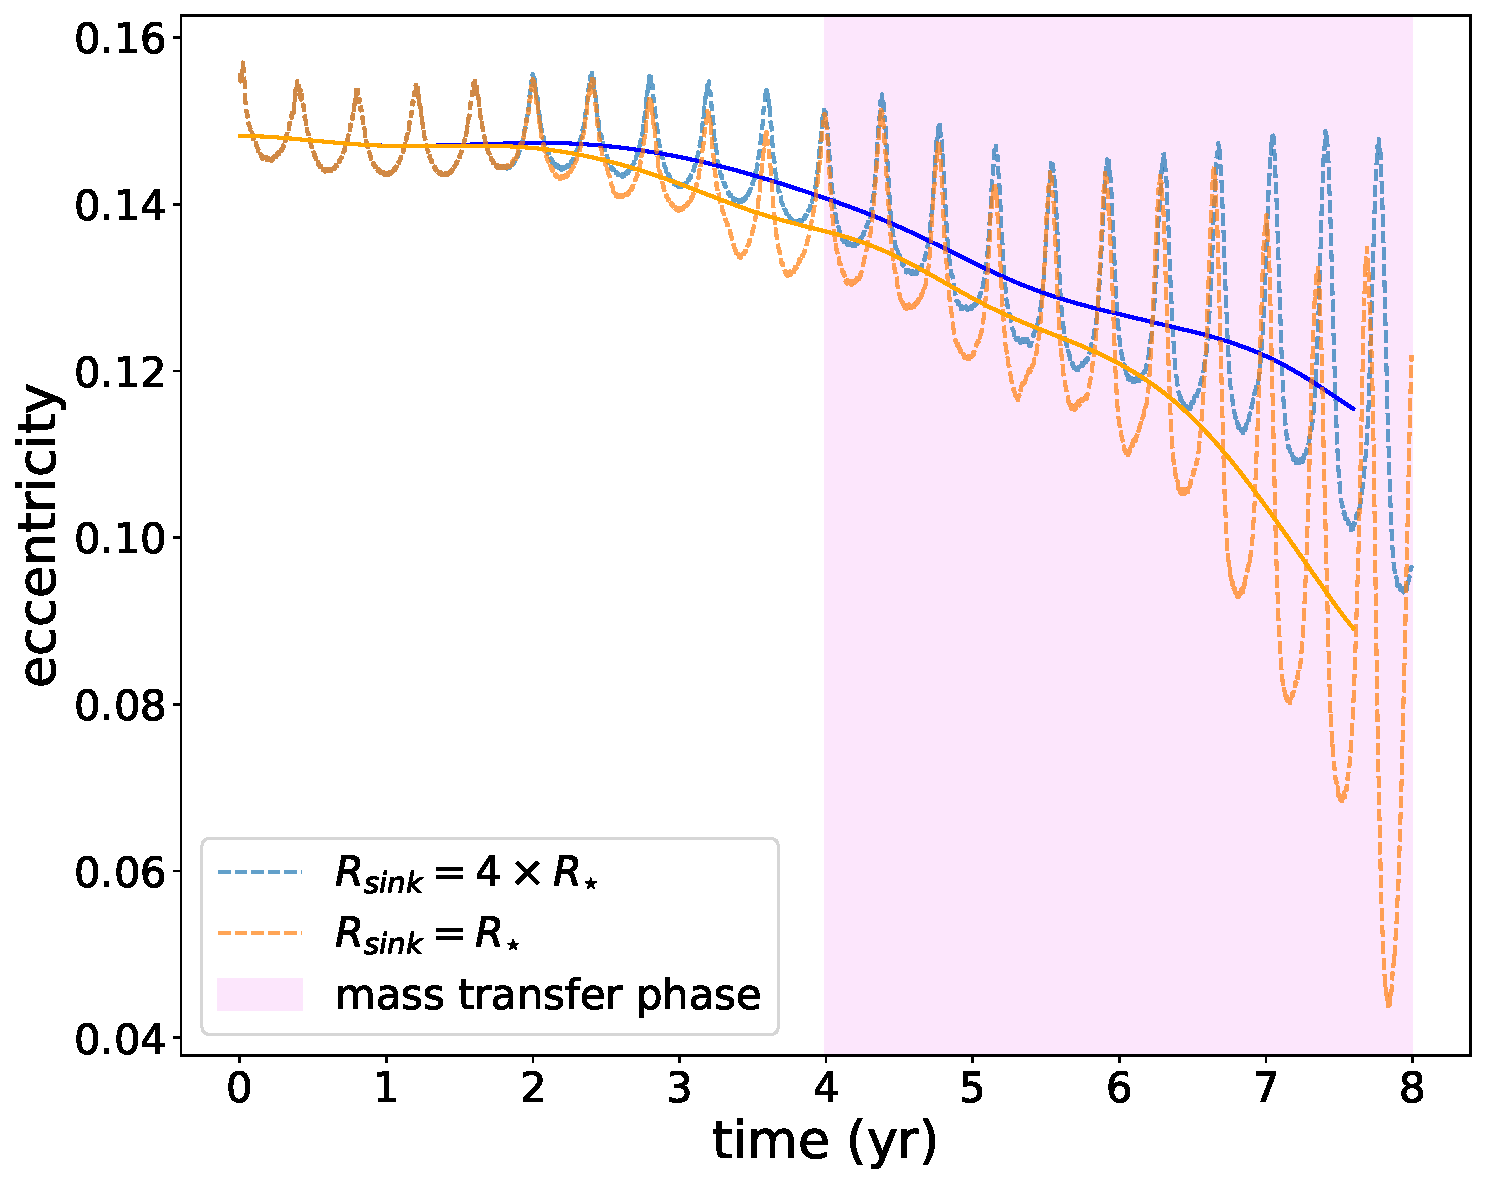
\includegraphics[width=0.76\textwidth]{Thesis/graphs/accretion_case/accretion_outer_ecc.pdf}
    \caption{Evolution of the eccentricity of the outer orbit for the minimum and maximum accretion case. The simulated data is shown in dashed lines. The continues lines are smooth representations of the simulated data in their respective colors. The last three orbits are not included in the smoothed version, because the lack of data above $8$ yr will erroneously flatten the slopes.}
    \label{fig:accretion_outer_ecc}
\end{figure}
\begin{comment}
\begin{figure}[H]
    \centering
    \begin{subfigure}{.5\textwidth}
    \centering
    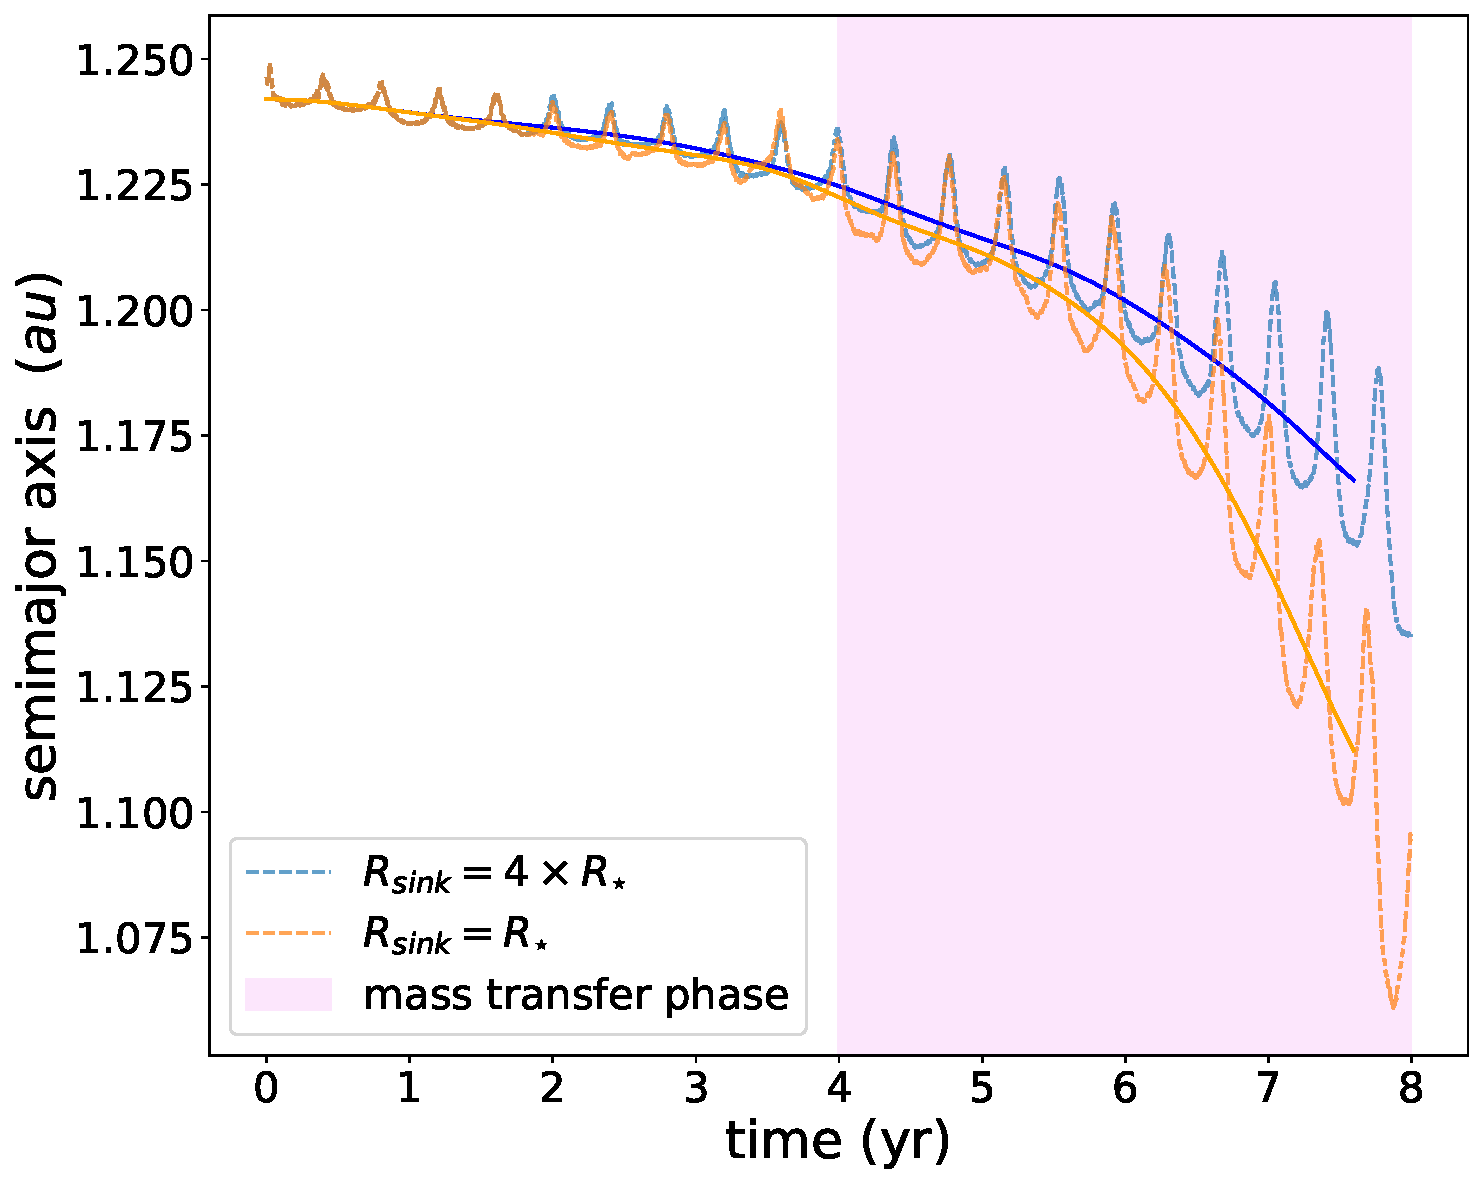
\includegraphics[width=0.9\textwidth]{Thesis/graphs/accretion_case/accretion_outer_semimajor_axis.pdf}
    \end{subfigure}%
    \begin{subfigure}{.5\textwidth}
    \centering
    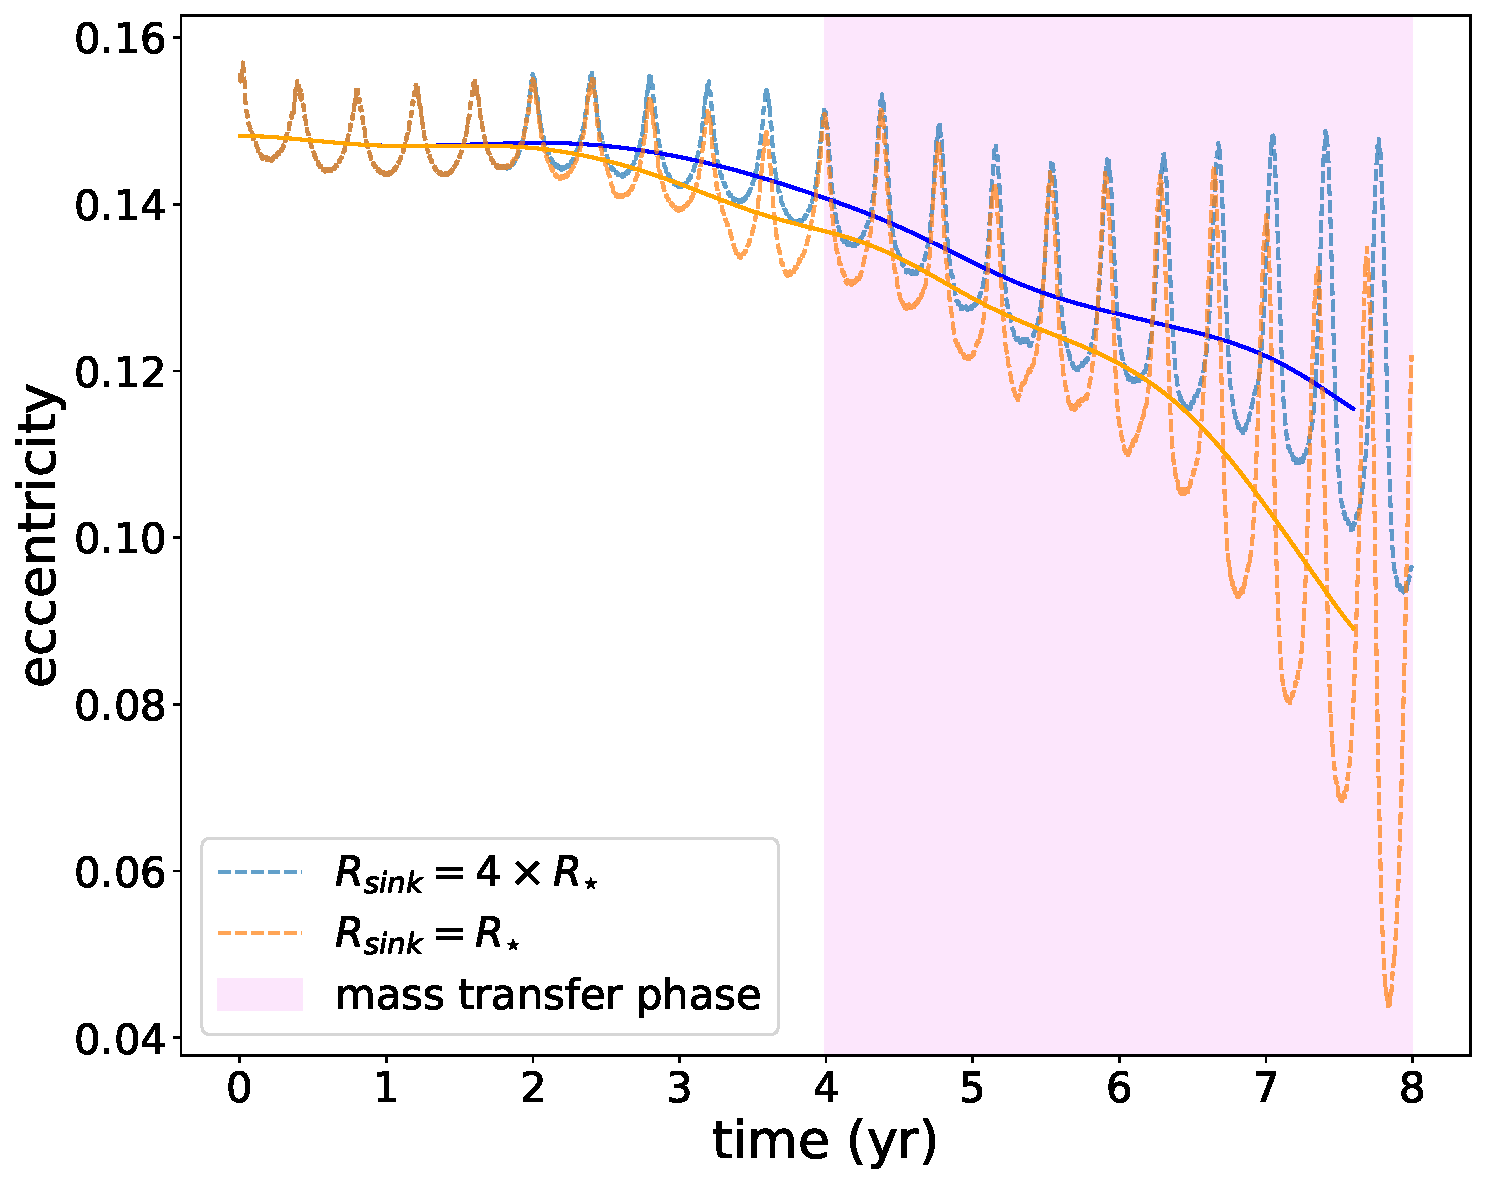
\includegraphics[width=0.9\textwidth]{Thesis/graphs/accretion_case/accretion_outer_ecc.pdf}
    \end{subfigure}
    \caption{ Evolution of the semi-major axis (left) and eccentricity (right) of the outer orbit}
    \label{fig:acc_outer_orbit}
\end{figure}
\end{comment}
\begin{figure}[!htb]
    \centering
    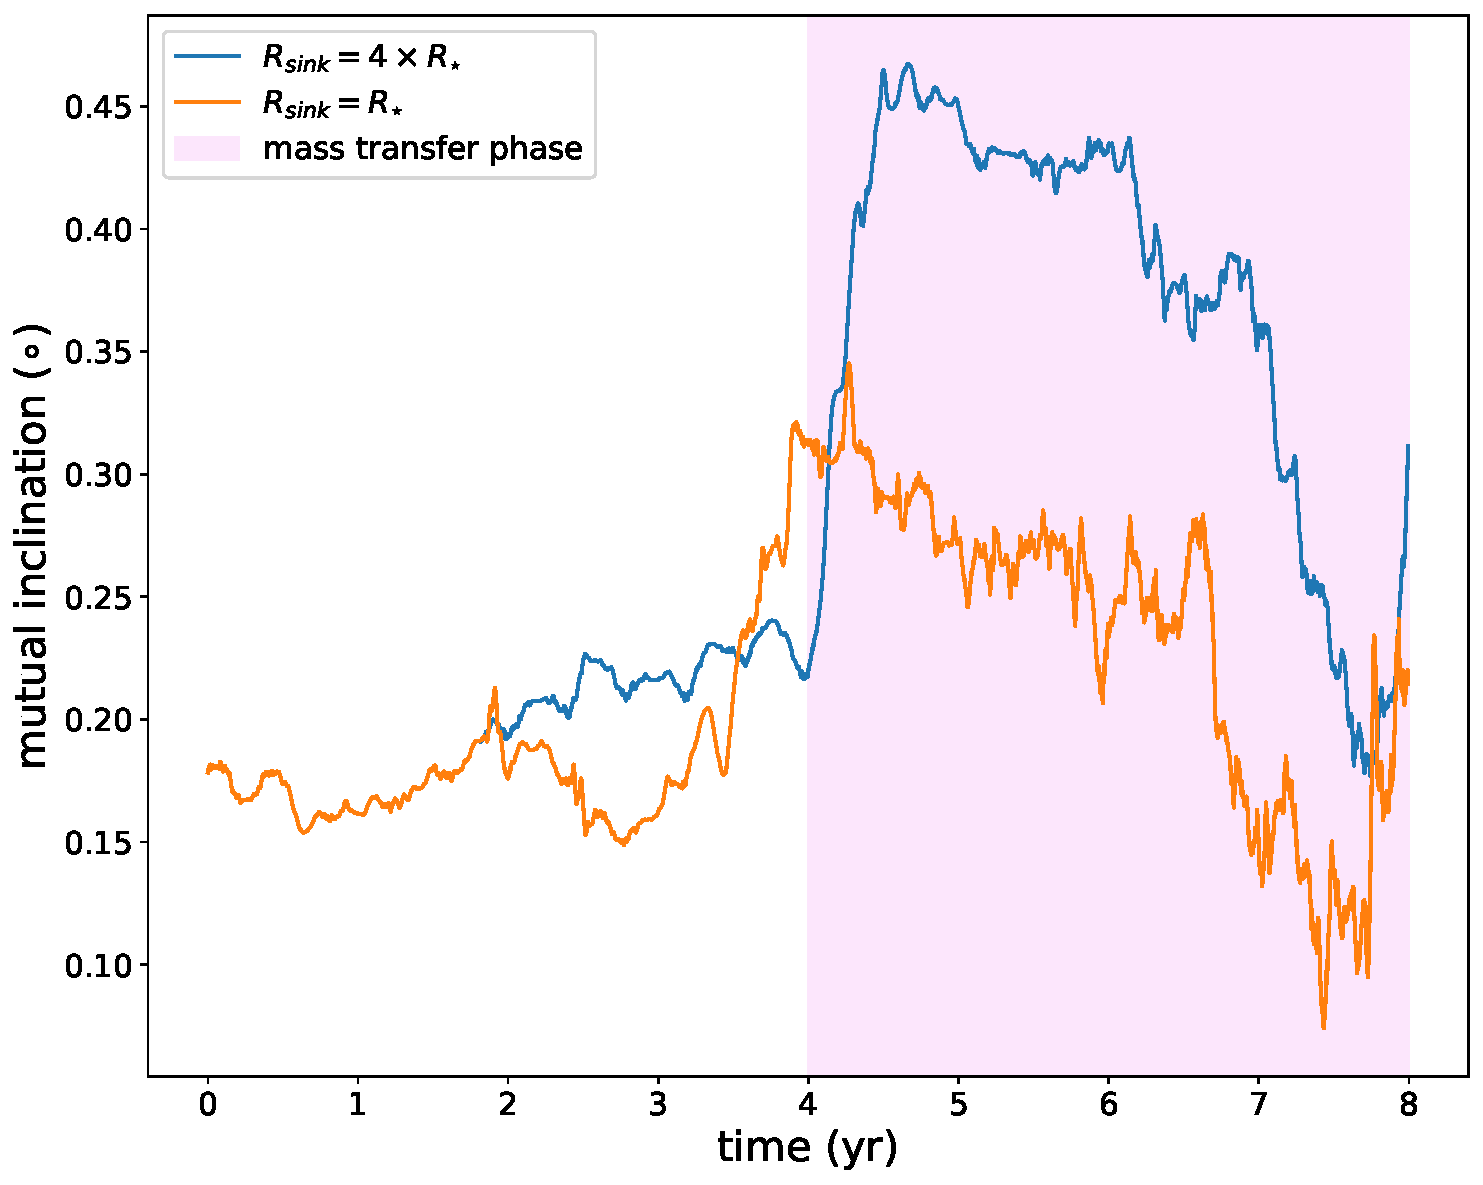
\includegraphics[width=0.76\textwidth]{Thesis/graphs/accretion_case/accretion_inc.pdf}
    \caption{Inclination of the outer orbit relative to the inner orbit.}
    \label{fig:accretion_inc}
\end{figure}
In \cref{fig:accretion_tertiary_mass}, I present the evolution of the tertiary's mass. The tertiary losses mass much faster in the minimum accretion case. The star's Roche lobe is proportional to its distance from the inner binary's center of mass; see \cref{eq:roche_lobe}, hence as the outer orbit decays faster, see \cref{fig:accretion_outer_semimajor_axis}, the tertiary's Roche lobe shrinks quicker. As a result, more and more gas overflows the Roche lobe and escapes towards the inner binary. To emphasize the difference in the mass evolution, I use central differentiation and provide mean mass loss rates for the simulated period, see \cref{fig:accretion_tertiary_mass}. The mass loss rates, should be taken with a grain of salt. Because the choice of $R_{\star} = 1.1 \times R_L$ significantly overestimates them, they should not be interpreted as average mass loss rates for RLOF, but they should be treated qualitatively. Despite that, it can not be ignored that the simulated values are in very good agreement with analytical ones calculated using \cref{eq:roche_lobe}.
\begin{figure}[H]
    \centering
    \begin{subfigure}{.5\textwidth}
    \centering
    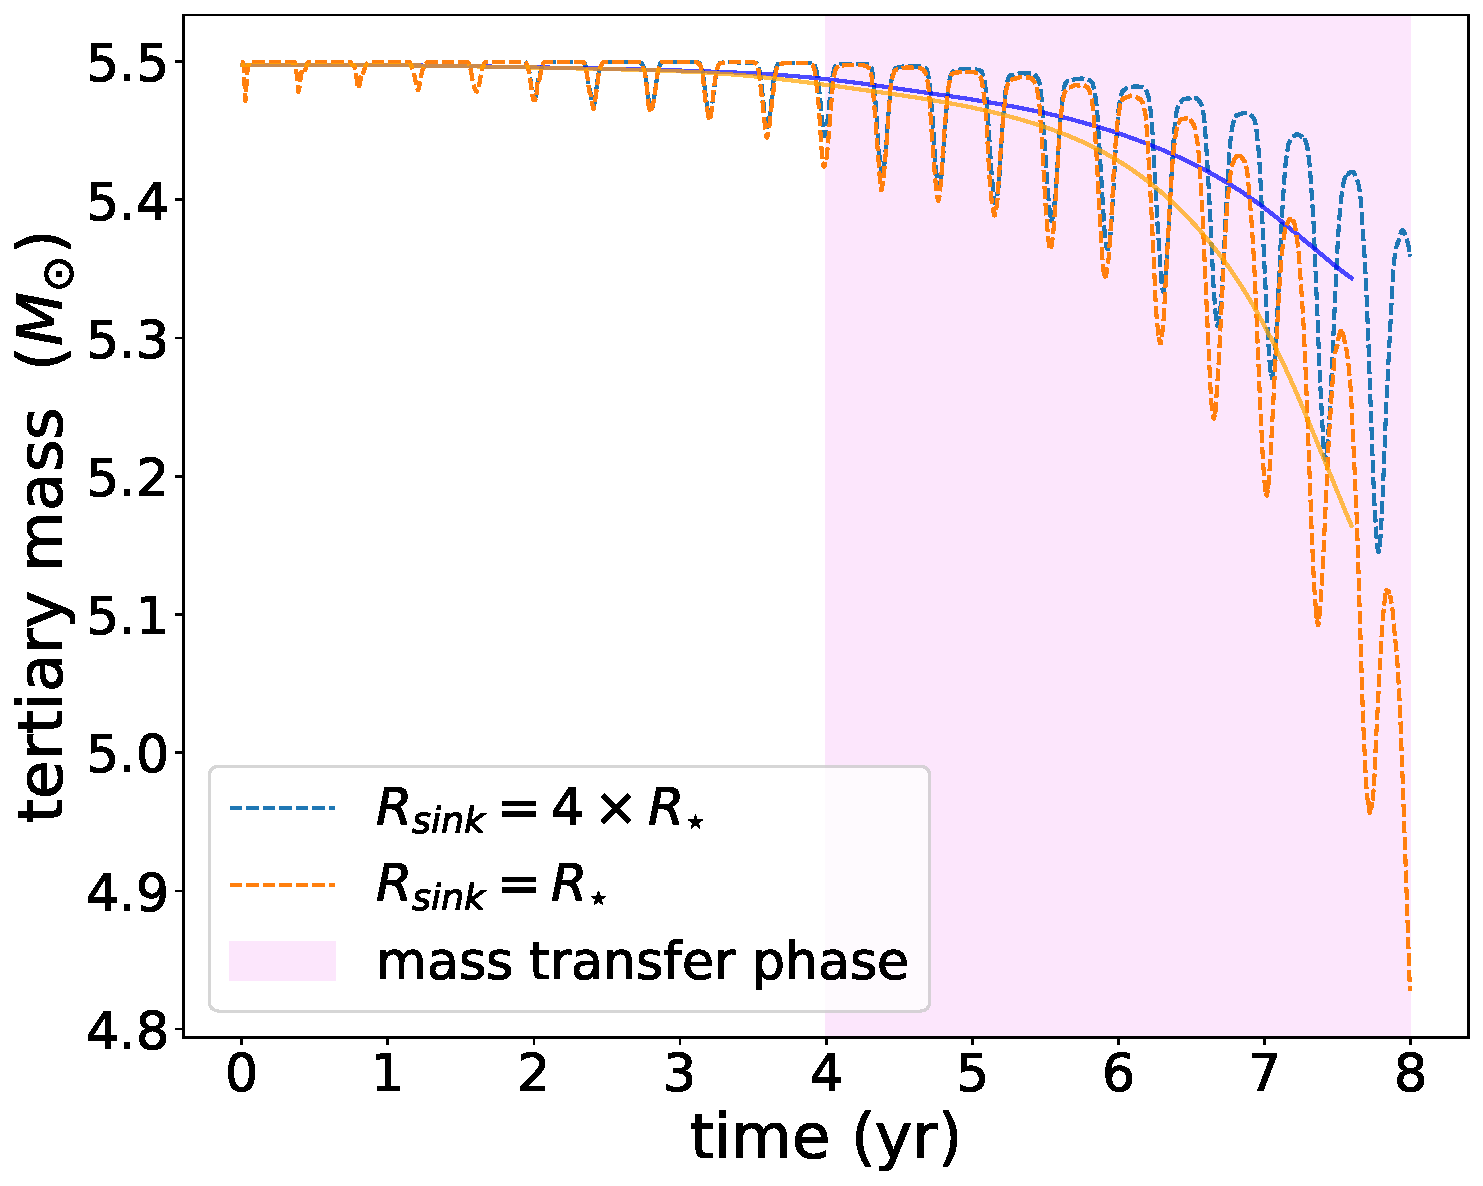
\includegraphics[width=0.9\textwidth]{Thesis/graphs/accretion_case/accretion_mass_loss.pdf}
    \end{subfigure}%
    \begin{subfigure}{.5\textwidth}
    \centering
    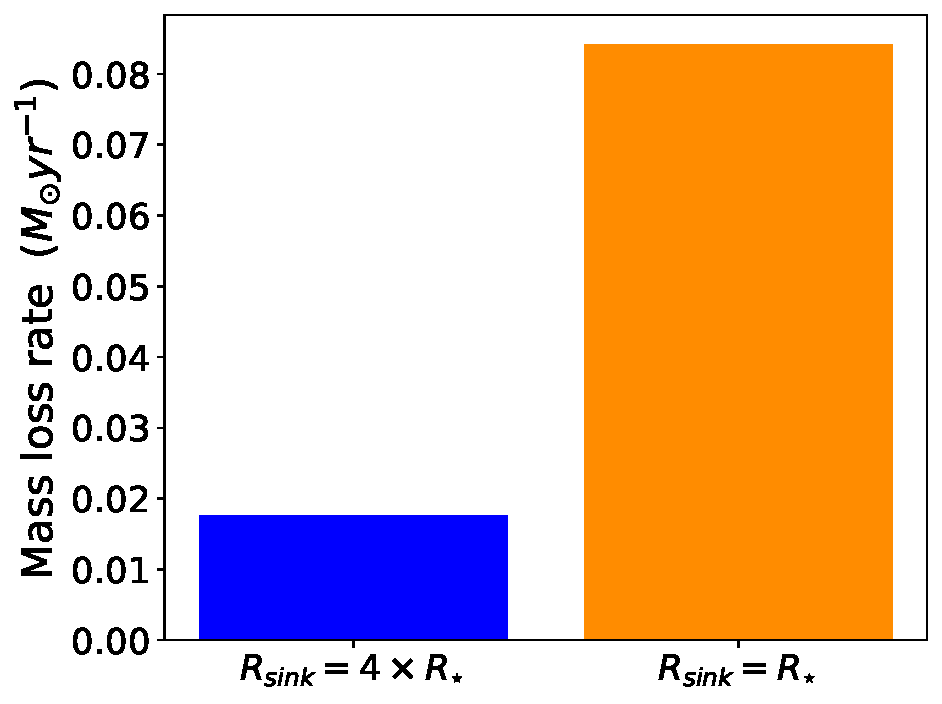
\includegraphics[width=0.9\textwidth]{Thesis/graphs/accretion_case/accretion_giant_mass_loss_rate.pdf}
    \end{subfigure}
    \caption{ The evolution of the tertiary's mass (left) for the minimum and maximum accretion case. The simulated data is shown in dashed lines. The continues lines are smooth representations of the simulated data in their respective colors. The last three orbits are not included in the smoothed version, because the lack of data above $8$ yr will erroneously flatten the slopes. The mean mass loss rates computed using central differentiation on the simulated data (right).}
    \label{fig:accretion_tertiary_mass}
\end{figure}


\subsection{Inner orbit}

In \cref{fig:accretion_inner_semimajor_axis} and \cref{fig:accretion_inner_ecc}, I present the evolution of the semi-major axis and eccentricity of the inner orbit, 
respectively. It is apparent that, the inner orbit widens in both the minimum and maximum accretion case. However, in the minimum accretion case, the orbit widens faster, see \cref{fig:accretion_inner_semimajor_axis}.
\begin{figure}[H]
    \centering
    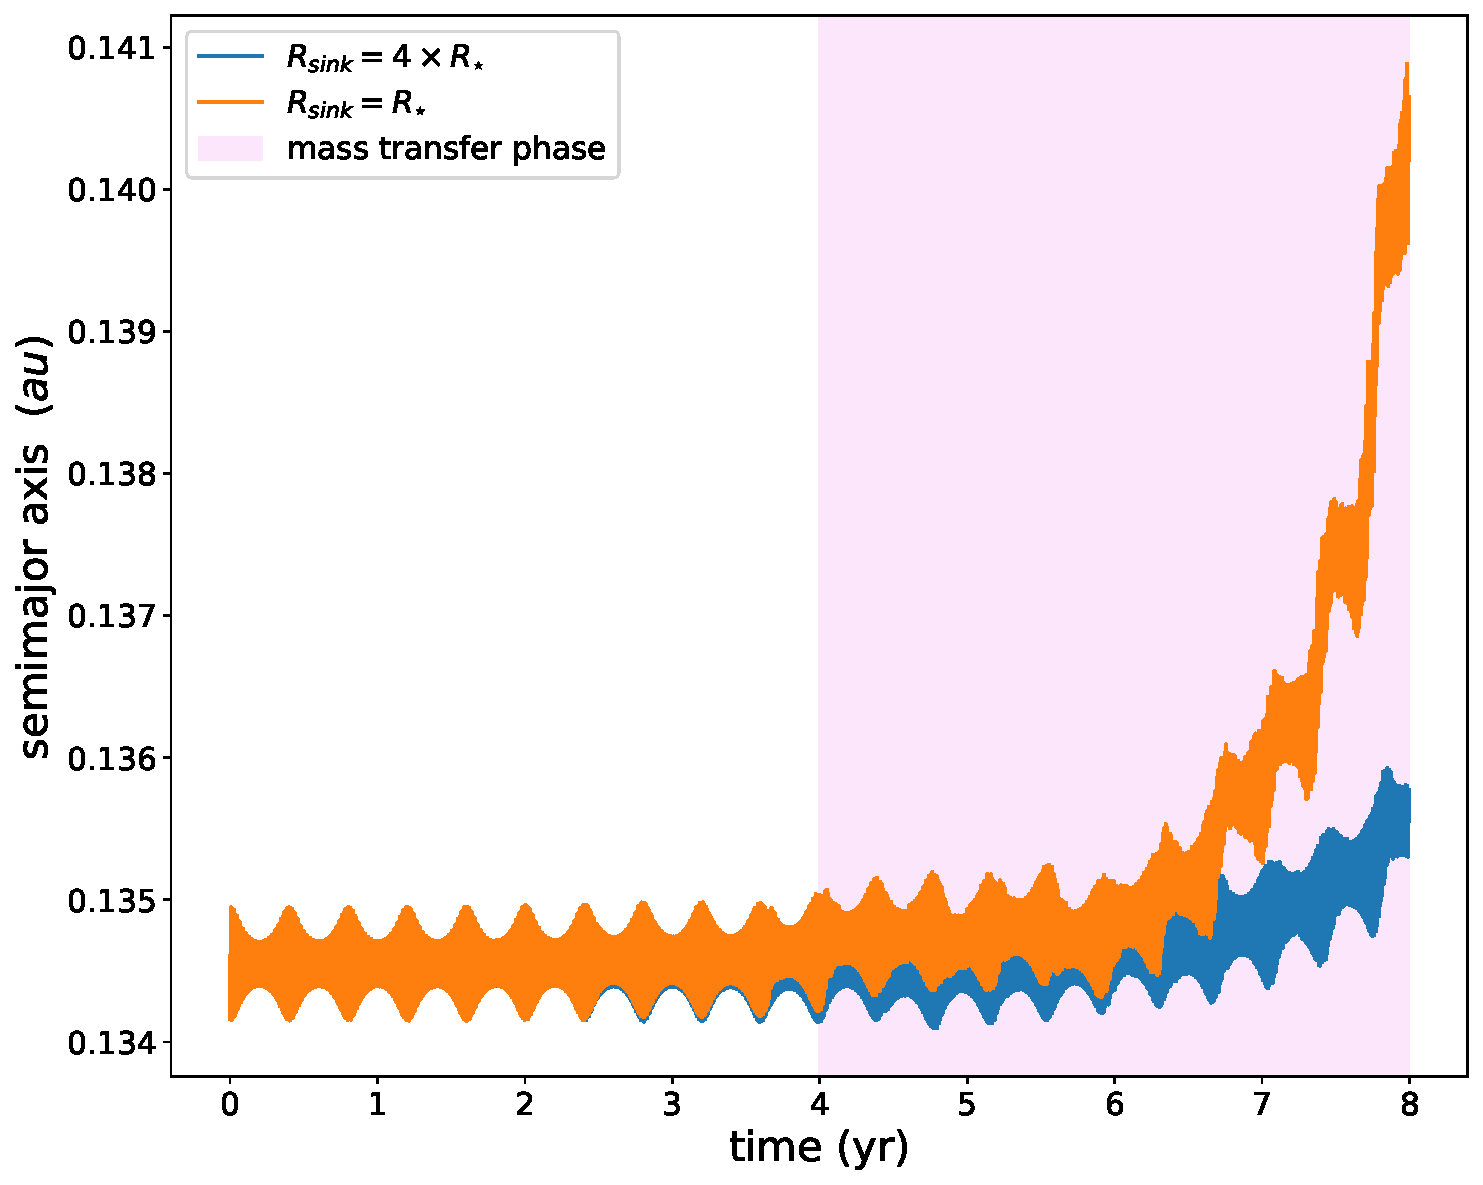
\includegraphics[width=0.9\textwidth]{Thesis/graphs/accretion_case/accretion_inner_semimajor_axis.pdf}
    \caption{Evolution of the semi-major axis of the inner orbit for the minimum and maximum accretion case.}
    \label{fig:accretion_inner_semimajor_axis}
\end{figure}
In the minimum accretion case, the tertiary's mass loss rate is much higher than the maximum accretion case, see \cref{fig:accretion_tertiary_mass} and the aforementioned trend is much more evident. Due to the underestimation of the effect of gas drag, the models are influenced by the gravitational interaction between the binary components and the incoming mass stream. The latter seems to result in a slingshot effect in favor of the the stars, see \cref{fig:retro} given that the orbital angular momentum of the inner and outer orbit are parallel. As more mass approaches the binary components, in the minimum accretion case, it can also approach them closer before it is being accreted, increasing the magnitude of the gravitational interactions. In conclusion, it is not possible to confidently draw conclusions about the impact of accretion on the inner orbit's semi-major axis given the current resolution. Finally, as expected, the effect of accretion on the eccentricity of the inner orbit is negligible. The orbit remains circular in both cases.
\begin{figure}[H]
    \centering
    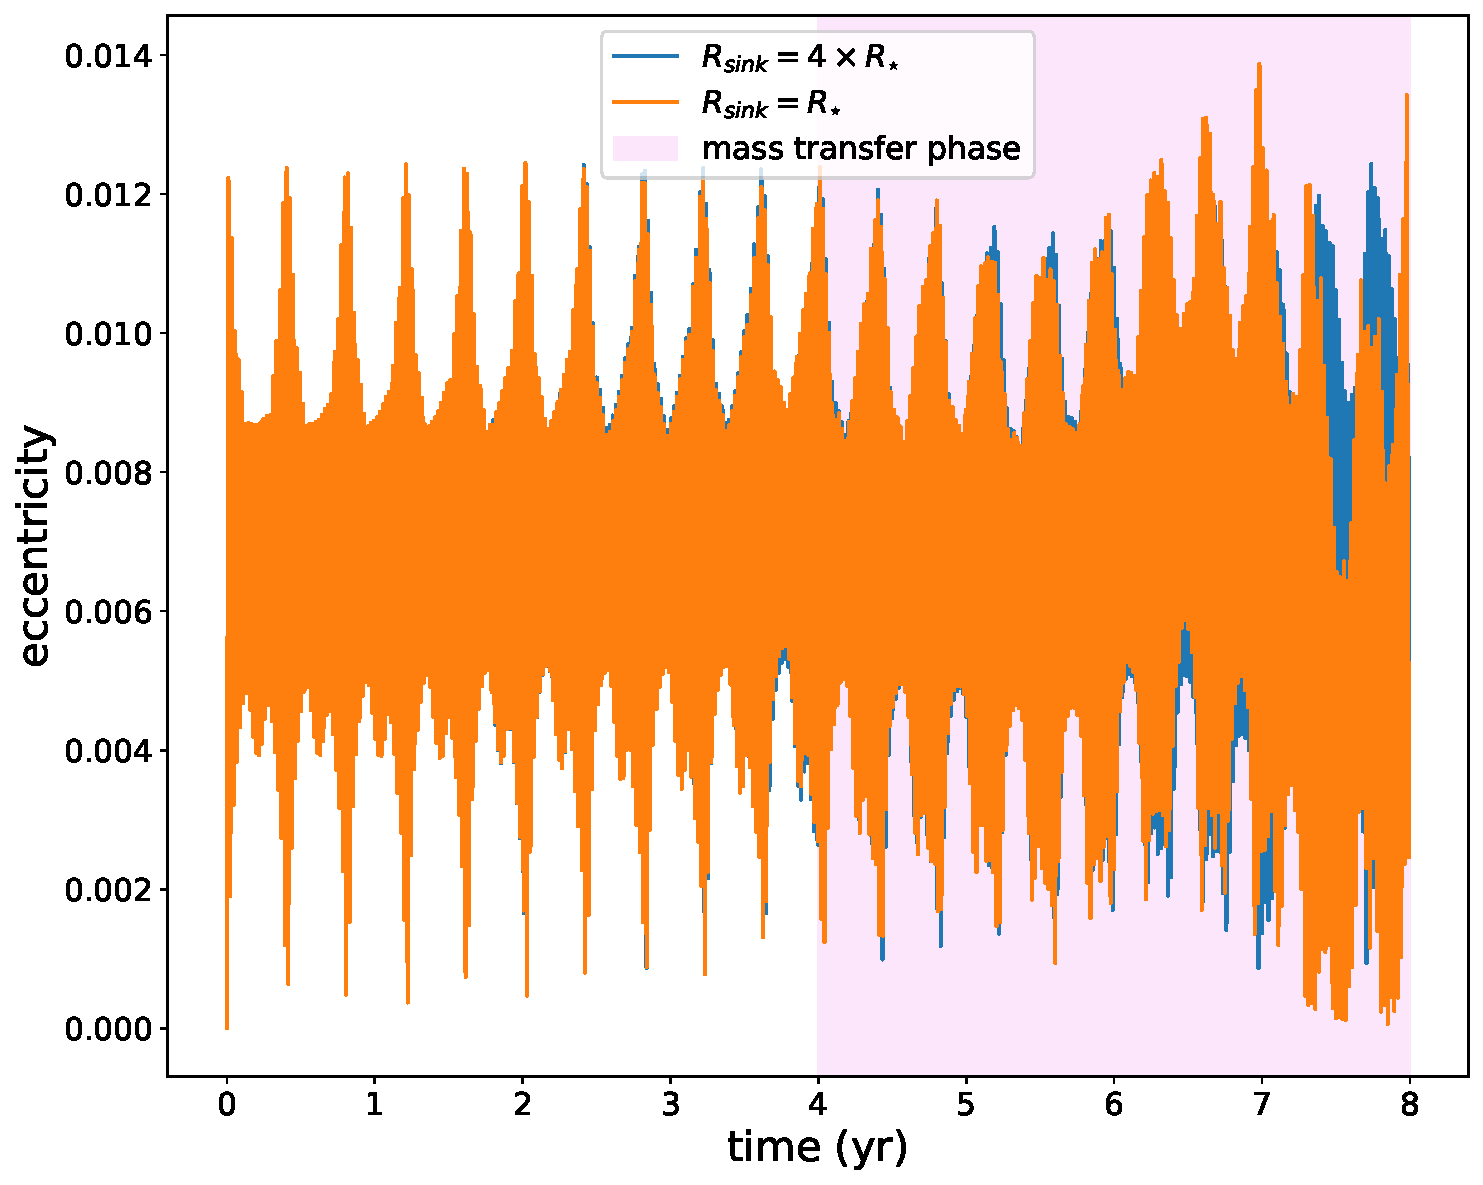
\includegraphics[width=0.9\textwidth]{Thesis/graphs/accretion_case/accretion_inner_ecc.pdf}
    \caption{Evolution of the eccentricity of the inner orbit for the minimum and maximum accretion case.}
    \label{fig:accretion_inner_ecc}
\end{figure}

\subsection{Analytical estimations}

During RLOF, matter from the outer donor star is either being accreted onto the inner binary stars, forms a disc around them, or is expelled from the triple system entirely. The orbits will change depending on what happens to the mass. This may be expressed in terms of the amount of angular momentum carried by the mass as it exits the donor star. On the one hand, the fraction of the accreted mass, $\beta$, and the amount of angular momentum that is carried away by the escaping mass are highly uncertain already in binary evolution studies. On the other hand, there are practically no theoretical predictions of the aforementioned quantities for mass transfer in hierarchical triples. More specifically, for the case of RLOF by an outer star towards the inner binary. 

In \cref{fig:accretion_eff_binary} I present an estimation of the accretion efficiency, $\beta$, for the maximum and minimum accretion case.
\begin{figure}[!htb]
    \centering
    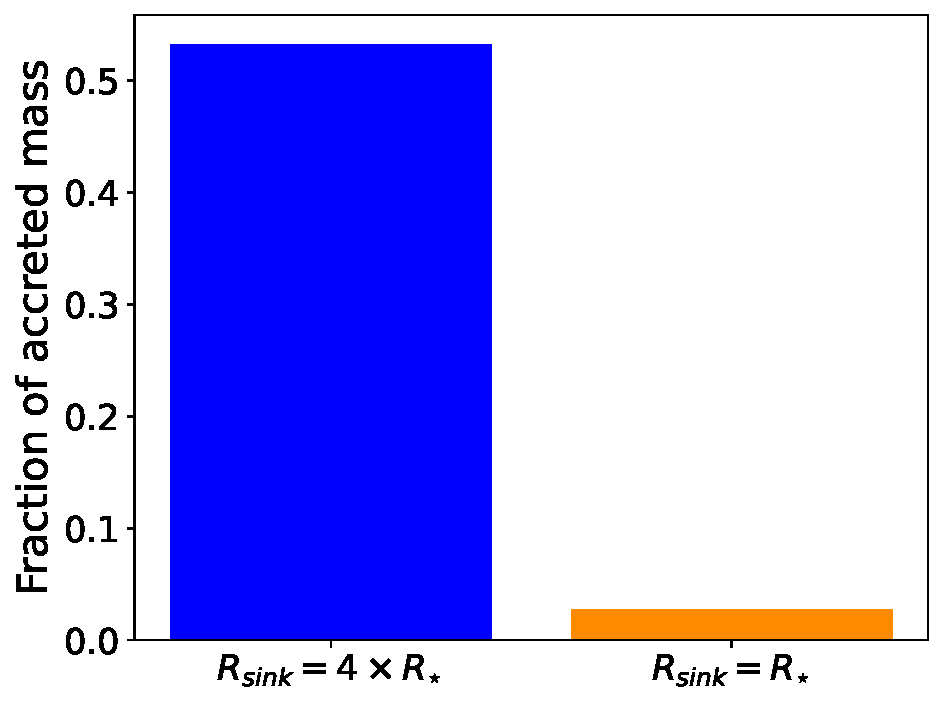
\includegraphics[width=0.9\textwidth]{Thesis/graphs/accretion_case/accretion_binary_acc_efficiency.pdf}
    \caption{Fraction of the accreted mass by the inner binary stars for the maximum and minim accretion cases.}
    \label{fig:accretion_eff_binary}
\end{figure}
In contrast to the concepts introduced in \cref{sub:orbit_evol_mass_loss}, $\beta$ corresponds to the fraction of mass being accreted by the inner binary. Nonetheless, $\beta = 0.53$ and $\beta = 0.03$ for the maximum and minimum accretion case, respectively. 

The absolute values presented, however, should be taken with a grain of salt. Higher resolution simulations are needed to examine the evolution of the inner semi-major axis, which may alter the details of the accretion process. Furthermore, the short period simulated here, can not capture additional parameters, which affect the fraction of accreted mass, $\beta$, such as the response of the accreting stars. The latter refers to the stars' envelope and rotational velocity response to the accreted mass. A more detailed discussion can be found in \cref{discussion}.

Despite the aforementioned uncertainties, the above outcome hints an intriguing possibility. The set up of the maximum accretion model intents to approach a conservative mass transfer scenario.
In \cite{zwart2019triple} study, the formation of a circumbinary disk leads to accretion efficiency up to $\beta \gtrsim 0.8$, despite the smaller accretion radii of the stars. In comparison, studies of conservative mass transfer in binaries report values of $\beta \geq 0.9$. As a result, it appears that, in the absence of a forming disk, the inner binary rotation makes accretion of incoming mass more difficult since part of it gets ejected via a slingshot effect. In conclusion, the accretion efficiency of the inner binary is most likely strongly related to whether or not a circumbinary disk forms. The absence of a forming disk suggests a highly non-conservative mass transfer.

On the one hand, the low resolution of the simulation and thus the underestimation of the gas drag does not allow for a direct comparison between analytical models and the evolution of the inner orbit's semi-major axis. On the other hand, the gas drag on the inner binary is mostly irrelevant for the evolution of the semi-major axis of the outer orbit, thus the amount of the lost angular momentum can be parameterized using analytical models.

In order to get an estimation about how much angular momentum is lost from the system, I compare the evolution of the semi-major axis of the outer orbit with the analytical model for non-conservative mass tranfer based on mass redistribution, see \cref{eq:semimajor_axis_no_cons}. The model assumes conservation of angular momentum despite the non-conservative case, similar to binaries as discussed by \cite{portegies1995formation}. Furthermore, it is assumed that the binary components are orbiting on the same plane, thus I compare the analytical model only with the models where $i_{mut}=0^{\circ}$, see \cref{tab:simulations_settings}.

Due to the fact that one component of the outer orbit is a binary system, the $M_a$ corresponds to its combined mass and $\eta$ is the specific angular momentum of the mass leaving the system as a proportion of the inner binary system's specific angular momentum. 
\begin{figure}[!htb]
    \centering
    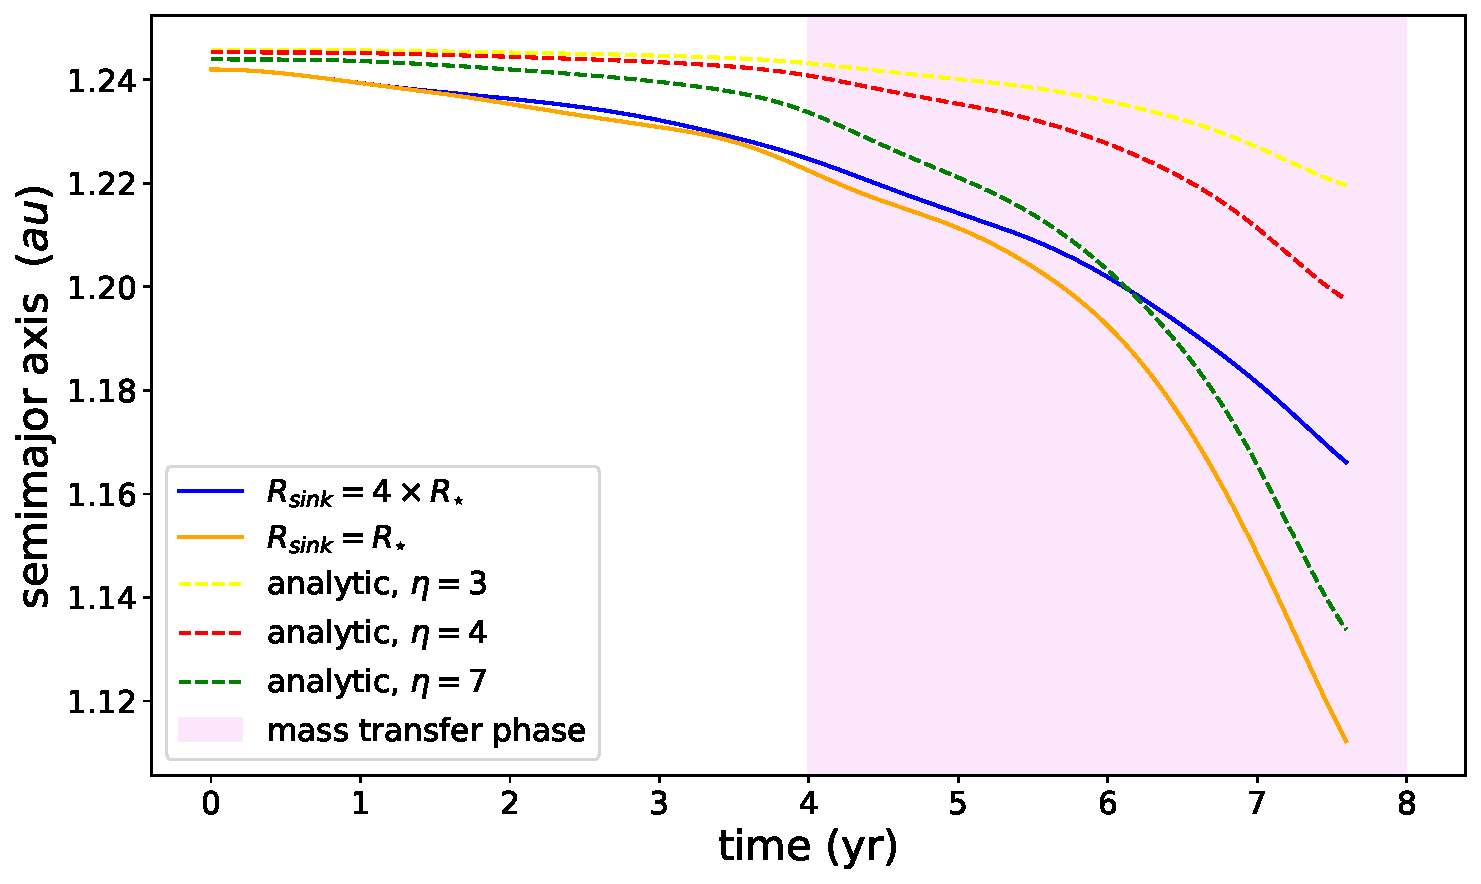
\includegraphics[width=0.85\textwidth]{Thesis/graphs/analytical_model.pdf}
    \caption{Evolution of the semi-major axis of the outer orbit for models number 1 and 4 listed in \cref{tab:simulations_settings}. The continues lines are representations of the simulated data, smoothed with a kernel with width $= 3 \times P_{out}$. The dashed lines correspond to analytical models in yellow, red, green and black, respectively.  The last three orbits are not included in the smoothed version, because the lack of data above $8$ yr will erroneously flatten the slopes.}
    \label{fig:comparison_analytical_model_max}
\end{figure}
In \cref{fig:comparison_analytical_model_max}, I present smoothed versions of the simulated data in blue and orange for the maximum and minimum accretion case, respectively. I also overplot four models, based on the maximum accretion case using \cref{eq:semi-major_axis}, for $\eta = 3,4,7,10$. Higher value of $\eta$ indicate that a higher amount of angular momentum is carried away by the ejected mass. During the mass transfer phase a model with $\eta \approx 4$ matches the slope of the orbital evolution for the maximum accretion case, while a model with $\eta \approx 7$ matches the minimum accretion case's orbital evolution slope. The graph indicates that in the maximum accretion case, given the same amount of ejected mass, the latter should carry significantly more angular momentum in order to match the minimum accretion case ($\eta = 7$). Hence, it is evident that the efficiency of the accretion process is vital for the timescale of the outer orbit's decay and consequently for the triple system's evolution.






\section{Impact of initial mutual inclination}\label{sec:inclination}


In this section, I investigate the importance of the initial mutual inclination on the evolution of the system. I present a comparison between simulations  1, 2 \& 3 listed in \cref{tab:simulations_settings}, which correspond to different initial inclination of the outer orbit relative to the inner orbit


\subsection{Outer orbit}

In \cref{fig:incliantion_tertiary_mass}, I present the evolution of the tertiary's mass for different initial mutual inclination. First, I would like to point out that the case of $i_{mut} = 69^{\circ}$ is not directly comparable to the other two cases. In order to place the tertiary initially at a higher inclination, the positions of all particles in the 3D model are corrected for the appropriate angle. Then the center of mass of the tertiary corresponds to the center of mass of all these particles. In this case, numerical rounding resulted into a shorter initial separation between the giant and the center of mass of the inner binary, see \cref{fig:inclination_outer_semimajor_axis}. More specifically, the tertiary was placed $\approx 0.01$ au ($\approx 2.15 R_{\odot}$) closer. This may seem as a small difference, but it has a significant impact on the mass loss rate. The smaller initial separation corresponds to higher fractional radius excess of the tertiary and considering \cref{eq:mass_loss_rate_anal}, the mass loss rate is highly overestimated in comparison with the other two models, see also \cref{fig:incliantion_tertiary_mass}.  As a result, the rate of decay of the outer orbit for the $i_{mut} = 69^{\circ}$ case is also overestimated compared to the other two models.
\begin{figure}[!htb]
    \centering
    \begin{subfigure}{.5\textwidth}
    \centering
    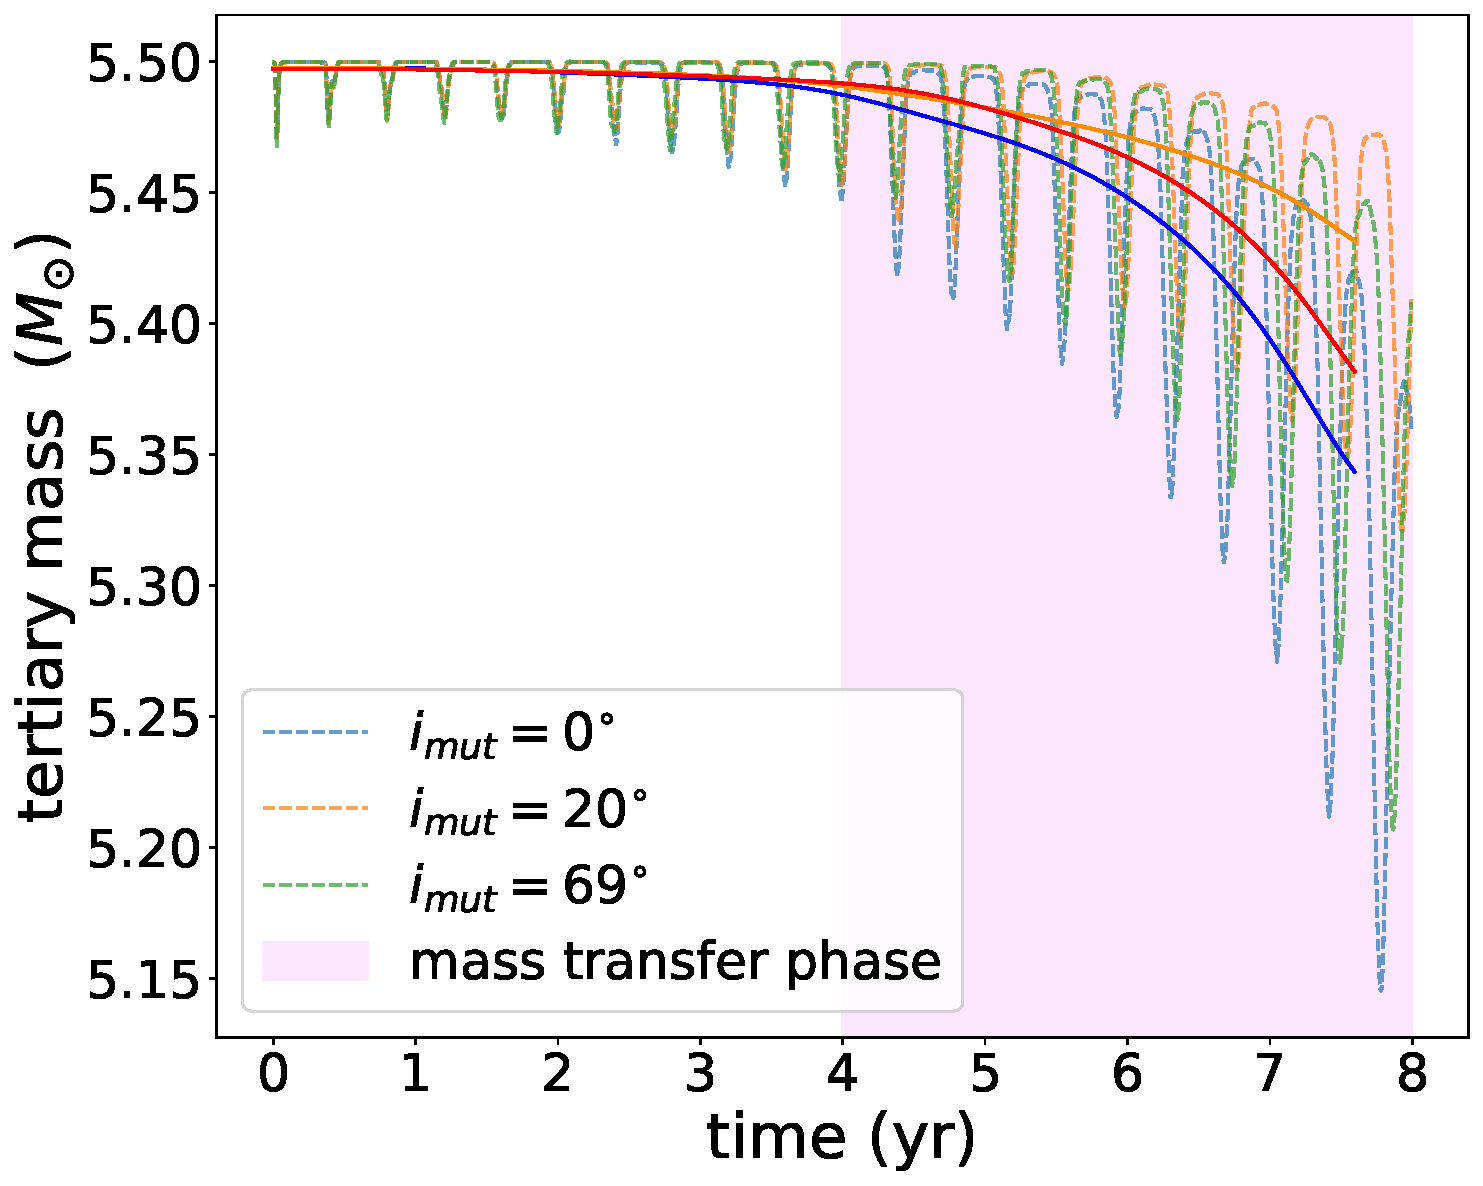
\includegraphics[width=0.9\textwidth]{Thesis/graphs/inclination_case/inclination_mass_loss.pdf}
    \end{subfigure}%
    \begin{subfigure}{.5\textwidth}
    \centering
    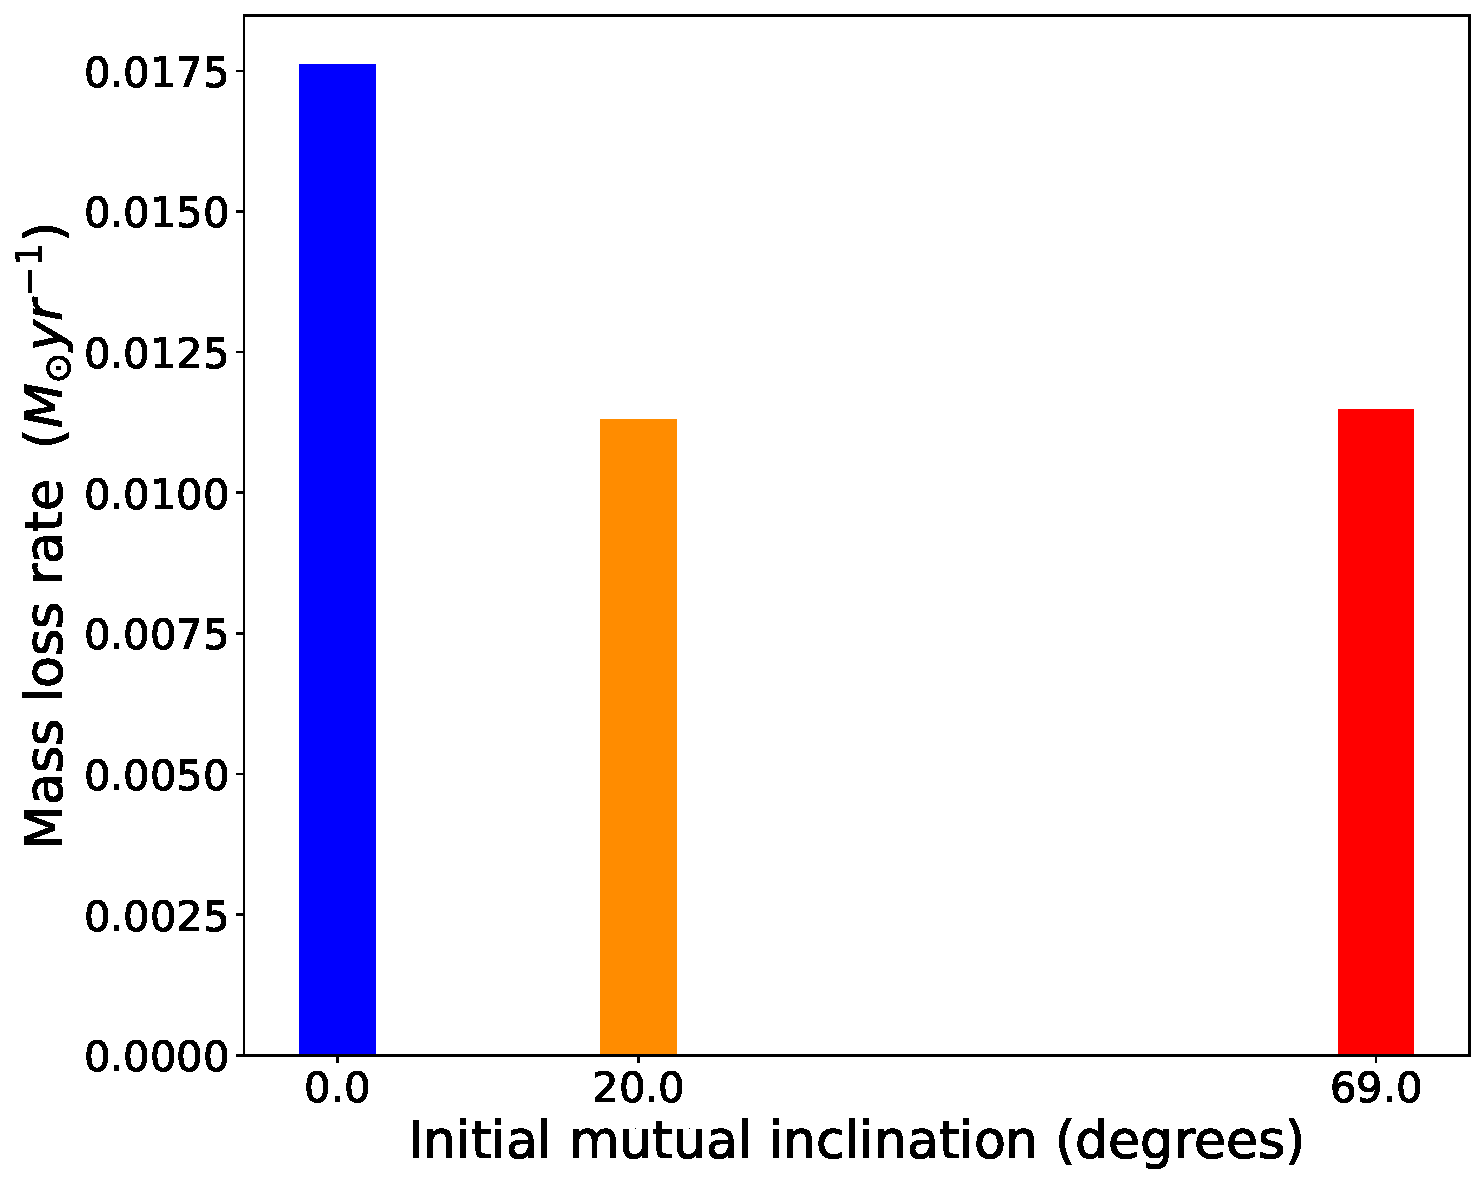
\includegraphics[width=0.9\textwidth]{Thesis/graphs/inclination_case/incliantion_giant_mass_loss_rate.pdf}
    \end{subfigure}
    \caption{ The evolution of the tertiary's mass (left) for of the outer orbit for different initial inclination of the outer orbit relative to the inner orbit. The simulated data is shown in dashed lines. The continues lines are smooth representations of the simulated data in their respective colors. The last three orbits are not included in the smoothed version, because the lack of data above $8$ yr will erroneously flatten the slopes. The mean mass loss rates computed using central differentiation on the simulated data (right).}
    \label{fig:incliantion_tertiary_mass}
\end{figure}

Keeping in mind that the mass loss rate for the case of $i_{mut} = 69^{\circ}$ is overestimated, I speculate that there is a trend: lower initial mutual inclination results to higher mass loss rate for the tertiary. This is not a surprise, as each of the inner binary stars can approach the giant closer for orbits that are nearly on the same plane. Additionally, the mass loss rate derived using central differentiation on the simulated data are in good agreement with the analytical ones calculated using \cref{eq:mass_loss_rate_anal}.
\begin{figure}[H]
    \centering
    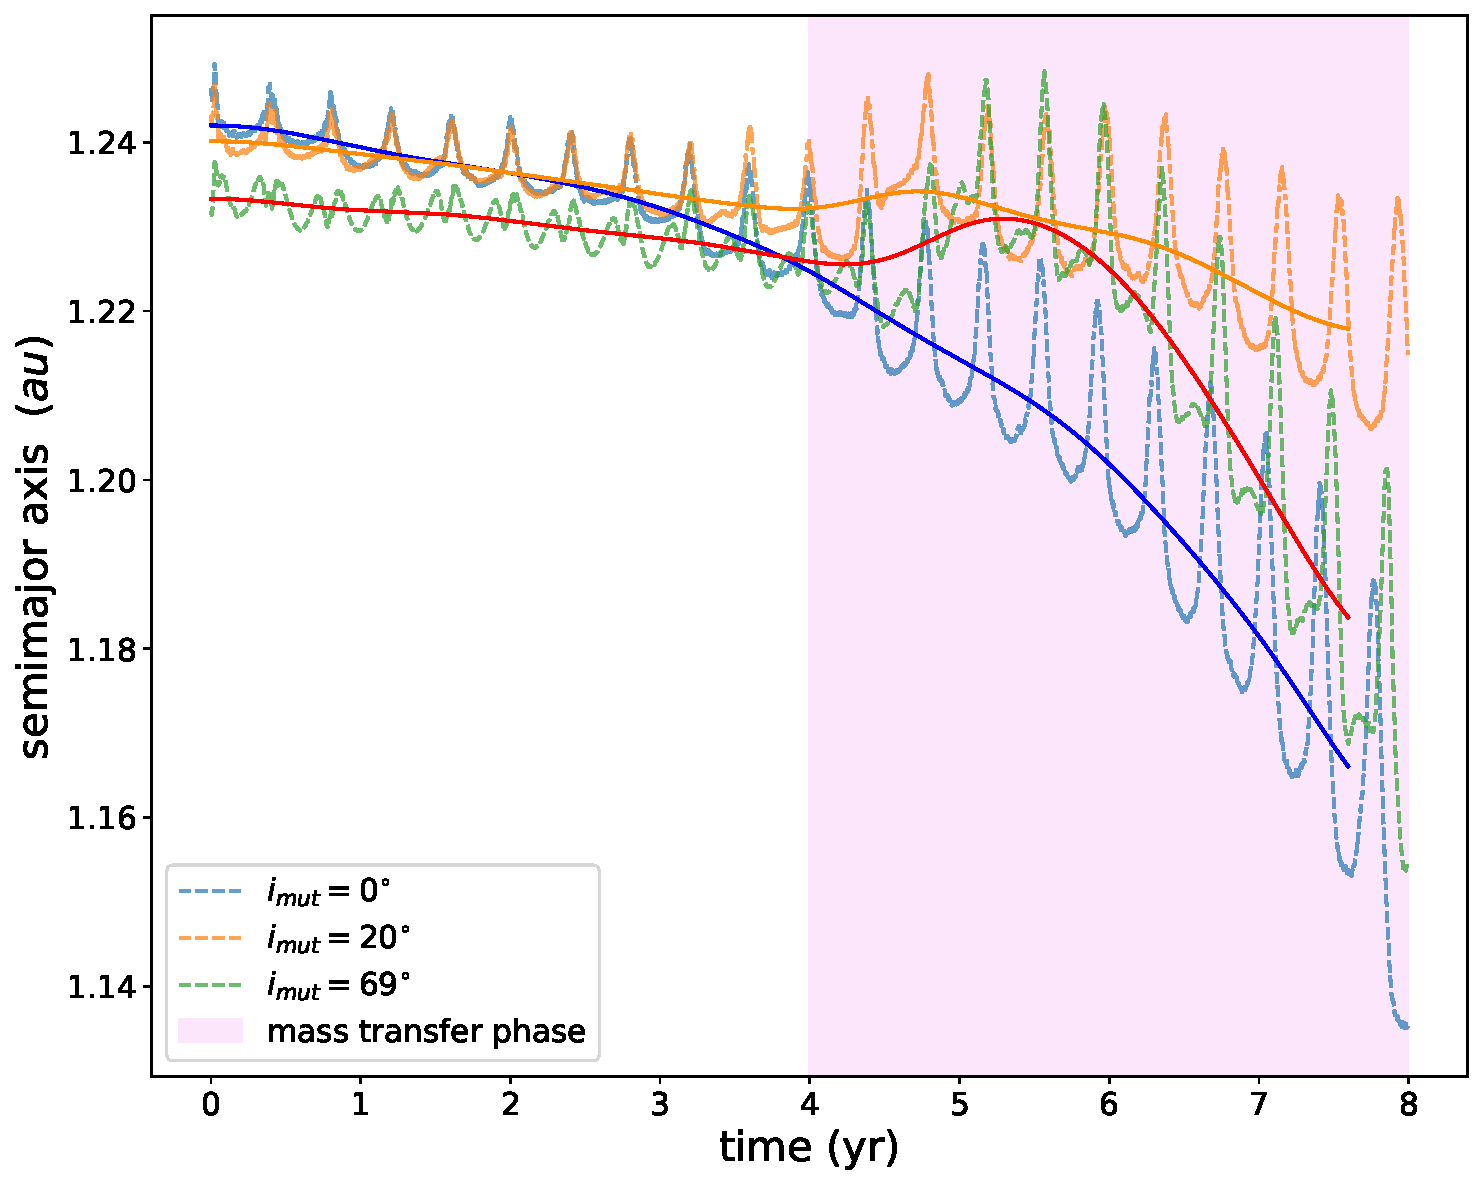
\includegraphics[width=0.85\textwidth]{Thesis/graphs/inclination_case/inclination_outer_semimajor_axis.pdf}
    \caption{Evolution of the semi-major axis of the outer orbit for different initial inclination of the outer orbit relative to the inner orbit. The simulated data is shown in dashed lines. The continues lines are smooth representations of the simulated data in their respective colors. The last three orbits are not included in the smoothed version, because the lack of data above $8$ yr will erroneously flatten the slopes.}
    \label{fig:inclination_outer_semimajor_axis}
\end{figure}
In \cref{fig:inclination_outer_semimajor_axis}, I display the evolution of the semi-major axis for different initial mutual inclinations. Considering only the $i_{mut} = 0^{\circ} \; \&  \; 20^{\circ}$ cases, the outer orbit decays faster for lower initial mutual inclination, because more mass is transferred towards the inner binary carrying away orbital angular momentum. 

In \cref{fig:inclination_outer_ecc},  the evolution of the eccentricity for different initial mutual inclinations is illustrated. Furthermore, in \cref{fig:mutual_inclination}, I present the evolution of the mutual inclination between the inner and the outer orbit for initial $i_{mut} = 20^{\circ}, 69^{\circ}$. The $i_{mut} = 0^{\circ}$ case is already displayed in \cref{fig:accretion_inc}.  Tidal interactions, as predicted, tend to circularize the outer orbit and also bring it towards coplanarity with the inner orbit.
\begin{figure}[H]
    \centering
    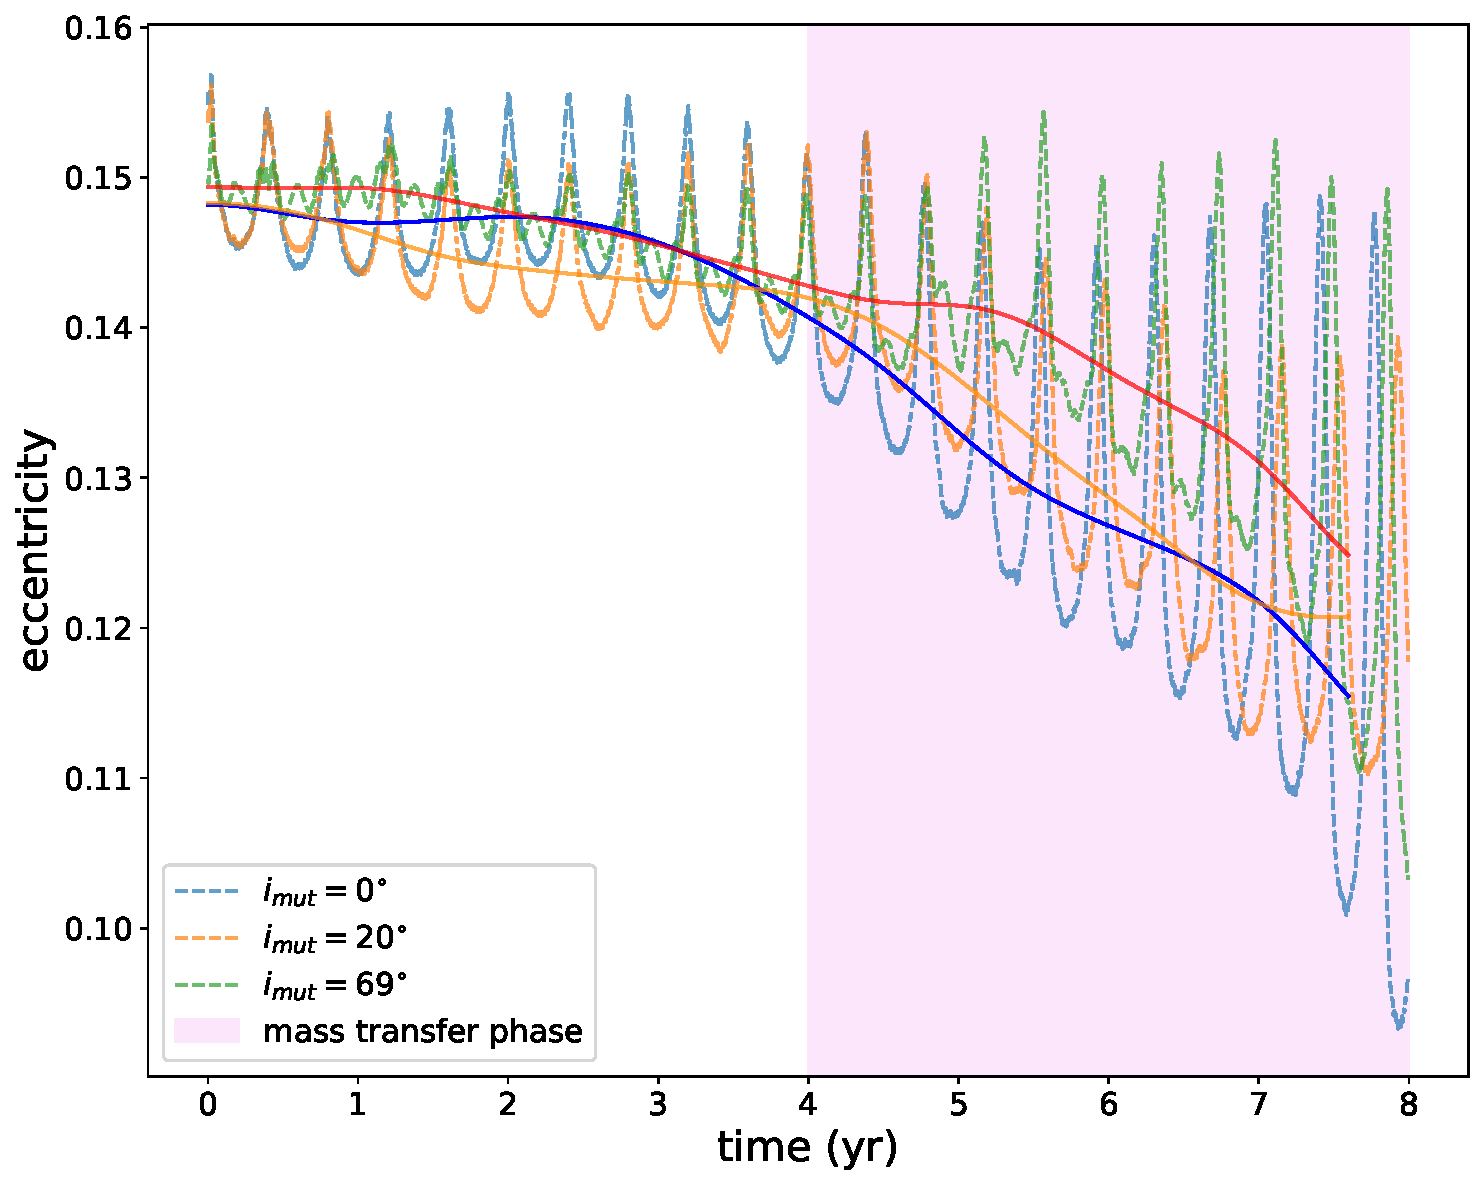
\includegraphics[width=0.9\textwidth]{Thesis/graphs/inclination_case/inclination_outer_ecc.pdf}
    \caption{Evolution of the eccentricity of the outer orbit for different initial inclination of the outer orbit relative to the inner orbit. The simulated data is shown in dashed lines. The continues lines are smooth representations of the simulated data in their respective colors. The last three orbits are not included in the smoothed version, because the lack of data above $8$ yr will erroneously flatten the slopes.}
    \label{fig:inclination_outer_ecc}
\end{figure}
As the giant, approaches the inner binary, the outer orbit tends to be circular, see \cref{fig:inclination_outer_ecc}. The interesting point though comes from a comparison between $i_{mut} = 20^{\circ} \& 69^{\circ}$. Despite the fact that for $i_{mut} = 69^{\circ}$ the giant has a higher mass loss rate and is closer $\sim 0.05$ au to the center of mass of the inner binary, see \cref{fig:inclination_outer_semimajor_axis}, the orbit circularizes faster for $i_{mut} = 20^{\circ}$. The individual inner binary stars can approach the giant closer for orbits that are nearly on the same plane, hence tidal interactions are expected to be stronger. The decay of the mutual inclination seems to be equivalent in both cases. The conclusion is that the effect of the hydrodynamics on the decay of the eccentricity and mutual inclination of the outer orbit is probably negligible. Both parameters are mostly affected by tidal interactions between the two orbits.
\begin{figure}[H]
    \centering
    \begin{subfigure}{.5\textwidth}
    \centering
    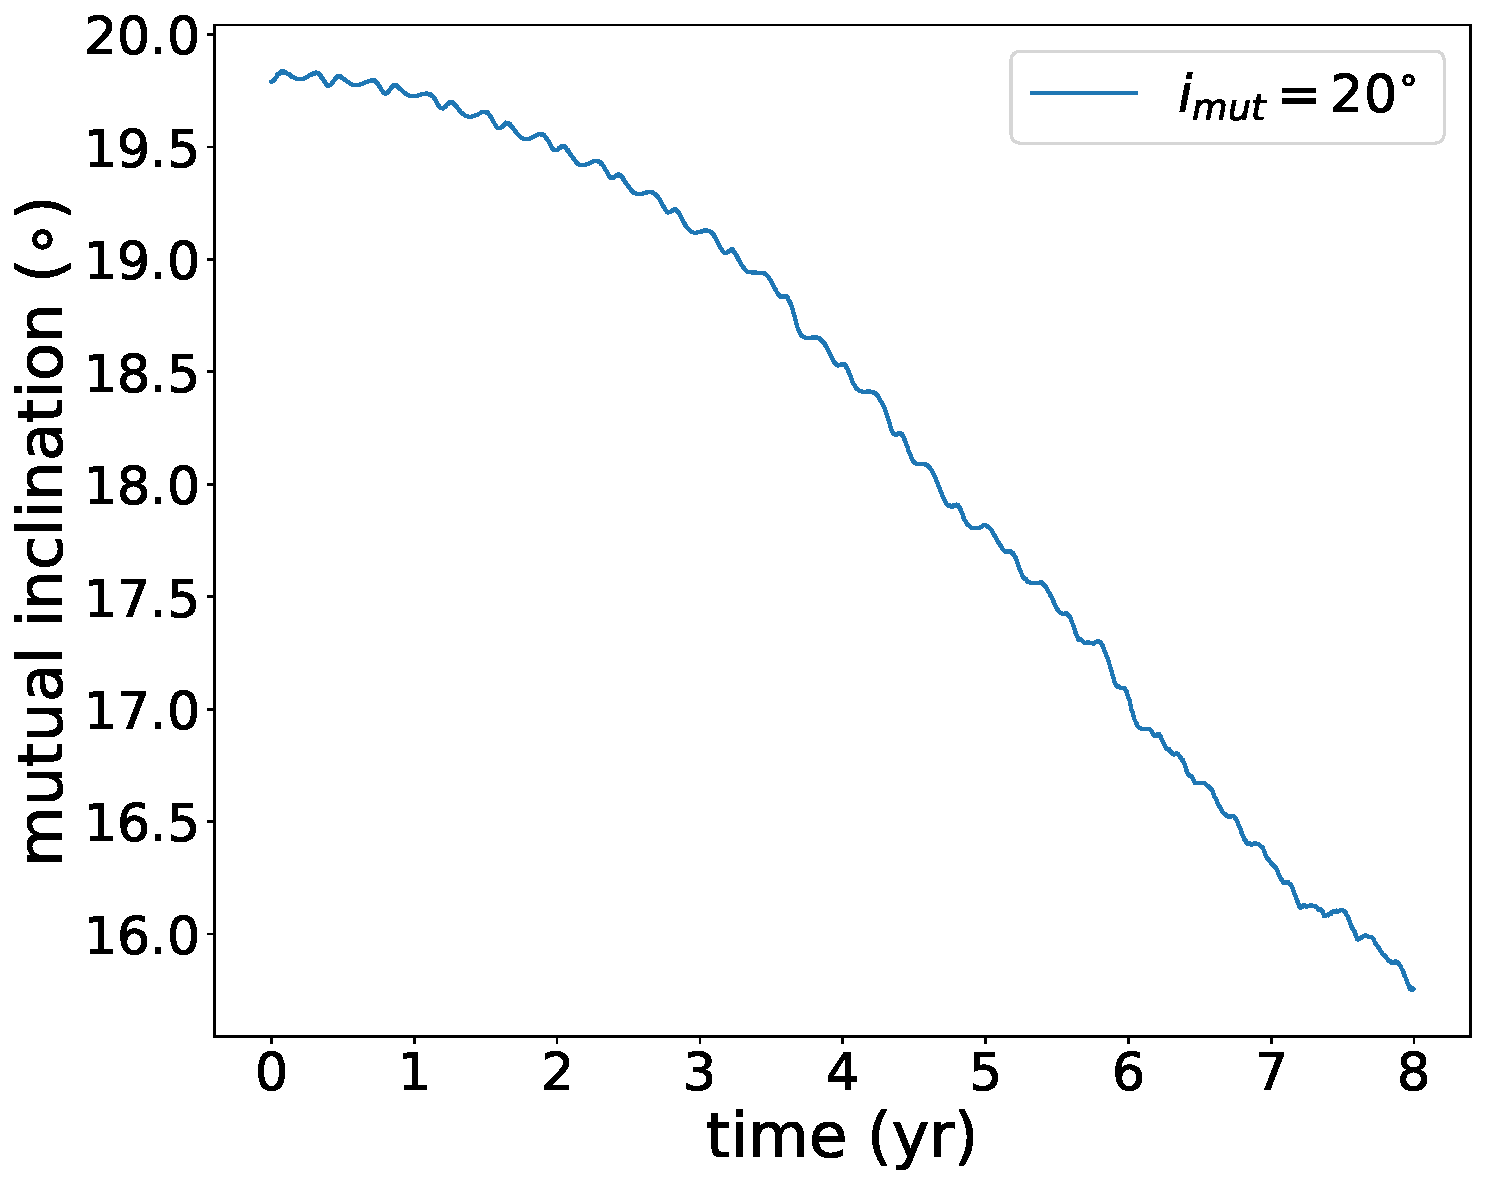
\includegraphics[width=0.9\textwidth]{Thesis/graphs/inclination_case/inc_20.pdf}
    \end{subfigure}%
    \begin{subfigure}{.5\textwidth}
    \centering
    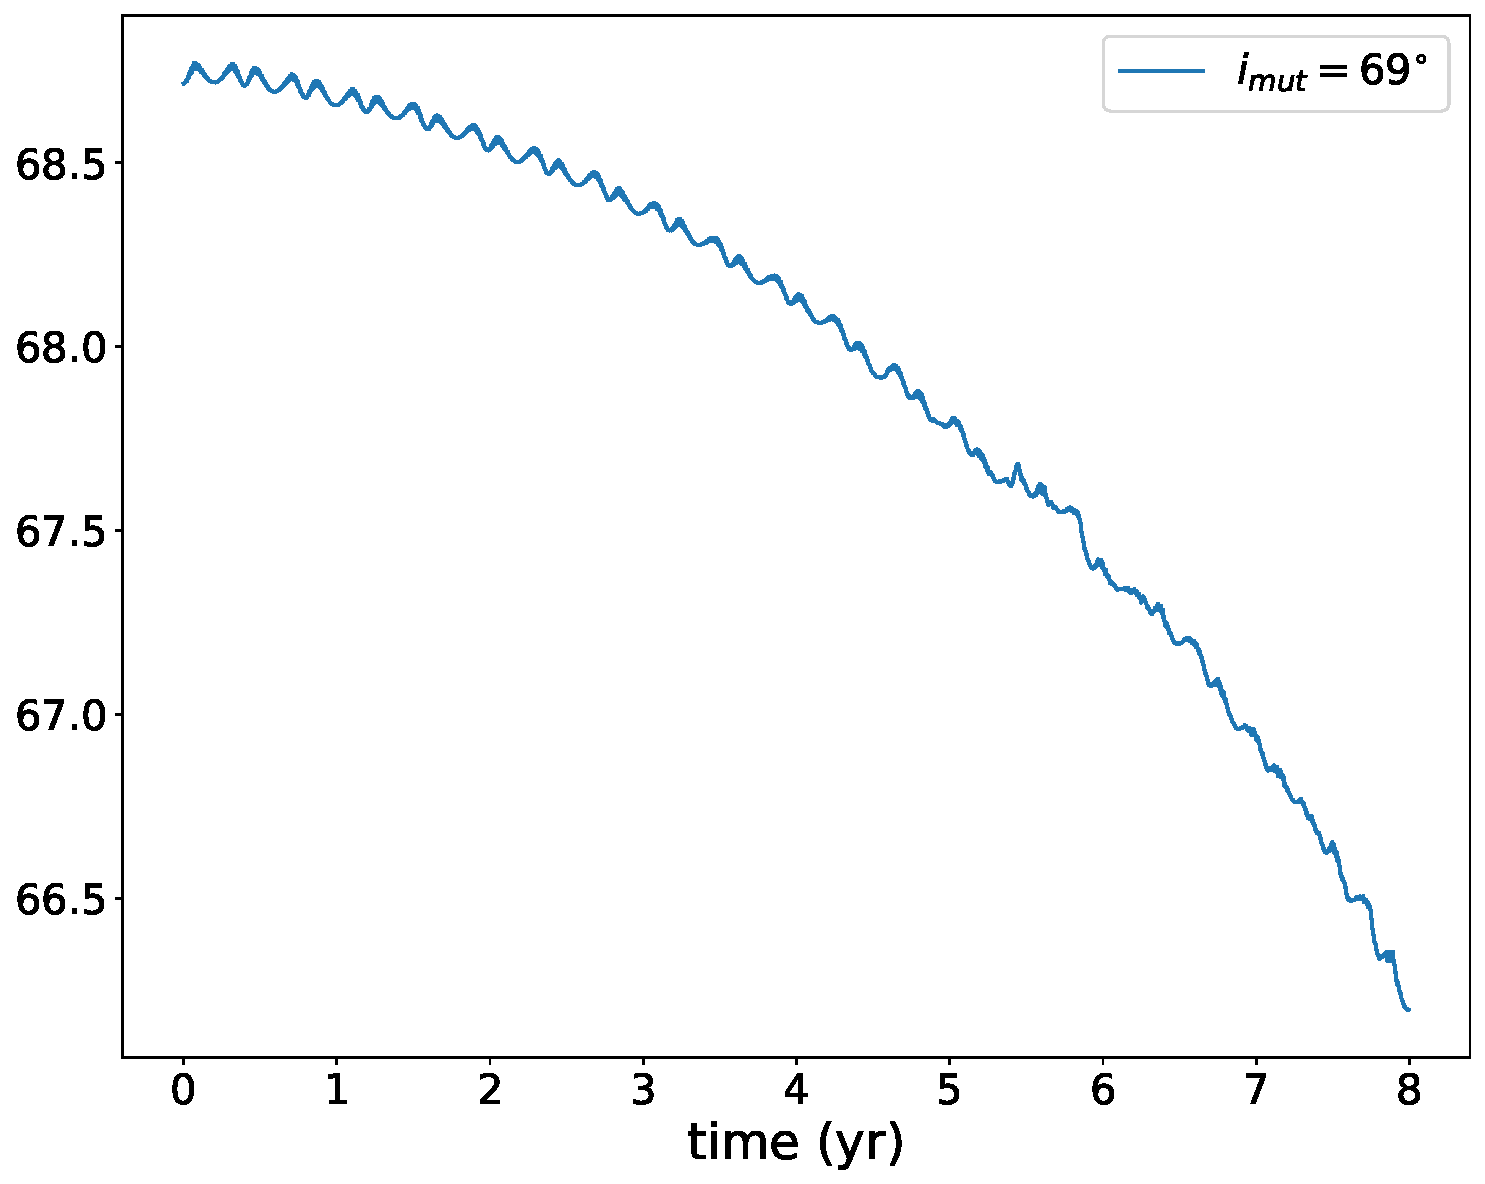
\includegraphics[width=0.9\textwidth]{Thesis/graphs/inclination_case/inc_69.pdf}
    \end{subfigure}
    \caption{ The evolution of the inclination of the outer orbit relative to the inner orbit for initial value: $i_{mut}=20^{\circ}$ (left) and $i_{mut}=69^{\circ}$ (right).}
    \label{fig:mutual_inclination}
\end{figure}

\subsection{Inner orbit}

In \cref{fig:inclination_inner_semimajor_axis} and \cref{fig:inclination_inner_ecc}, I present the evolution of the semi-major axis and eccentricity of the inner orbit for different initial mutual inclinations, respectively. The observed behavior for low inclinations, such as $i_{mut}=0^{\circ}, 20^{\circ}$, has already been described in \cref{sec:accretion}, but the case of $i_{mut}=69^{\circ}$ yields some intriguing results.

Despite underestimating the gas drag, it is evident that I can still extract some valuable insights regarding the evolution of the inner orbit. The inner orbit shrinks with the greatest initial mutual inclination. The reason for this behavior is that the mass stream can successfully cross the inner orbit at high angles, draining orbital angular momentum from the latter. Additionally, because gas drag always tends to shrink the orbit, the observed behavior is qualitatively accurate. The only difference is that including gas drag, the rate of the orbit's decay will be higher or in simple words the observed slope will be steeper. 
\begin{figure}[H]
    \centering
    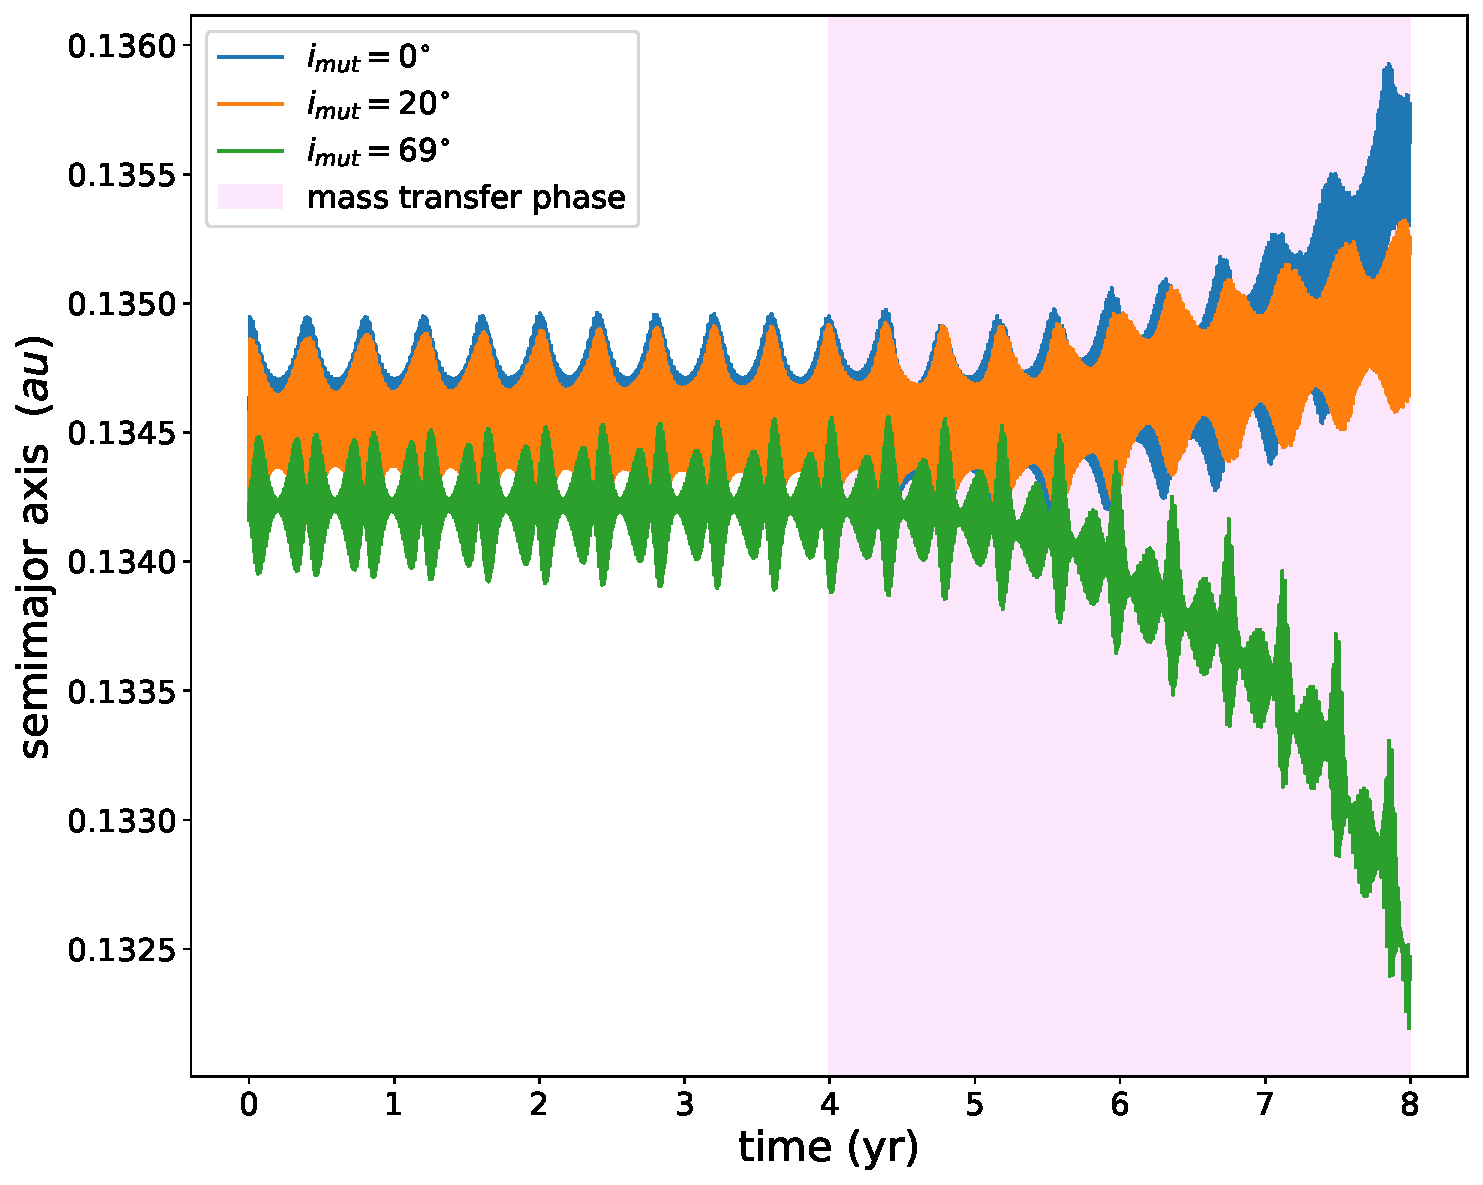
\includegraphics[width=0.9\textwidth]{Thesis/graphs/inclination_case/inclination_inner_semimajor_axis.pdf}
    \caption{Evolution of the semi-major axis of the inner orbit for different initial mutual inclination.}
    \label{fig:inclination_inner_semimajor_axis}
\end{figure}
The $i_{mut}=69^{\circ}$ value was selected intentionally, to test the accuracy of the coupled solver. It is clear, that the latter can resolve Lidov-Kozai cycles. The $i_{mut}=69^{\circ}$ is well inside in the regime where the Lidov-Kozai cycles are expected to occur, see \cref{sub:lidov_kozai}. The eccentricity and mutual inclination are expected to vary periodically. As expected, as the eccentricity increases and the mutual inclination decreases, see \cref{fig:mutual_inclination} and \cref{fig:inclination_inner_semimajor_axis}.
\begin{figure}[!htb]
    \centering
    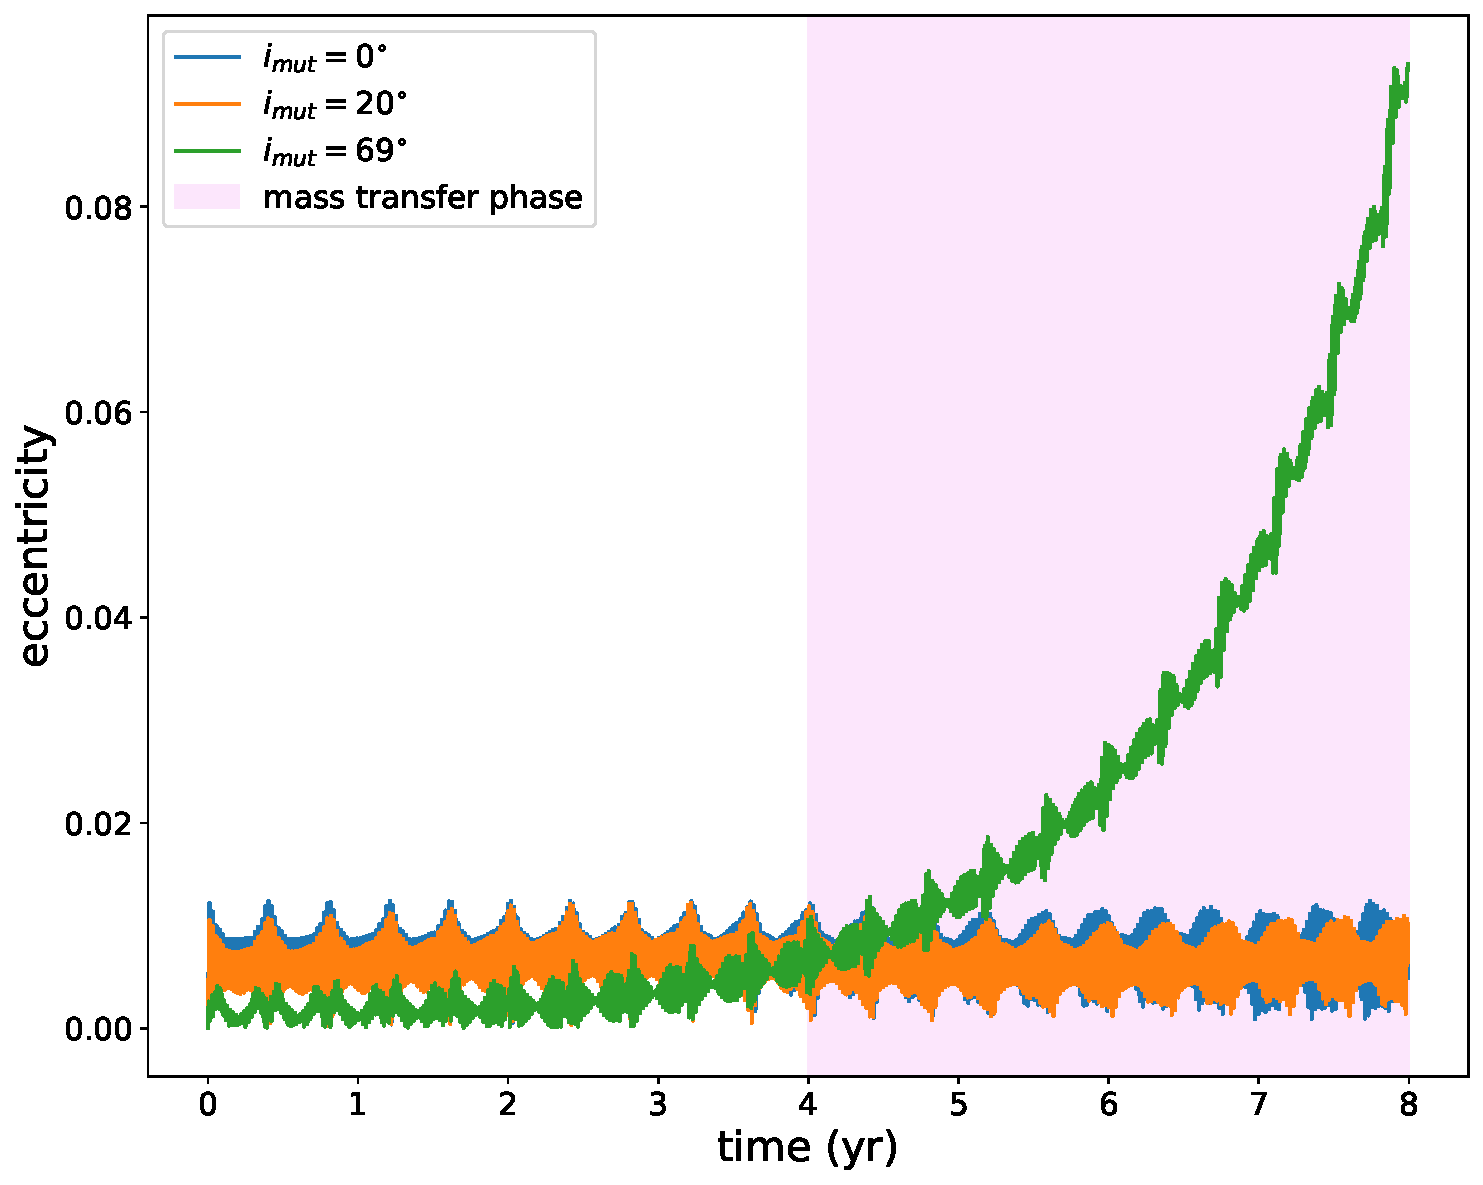
\includegraphics[width=0.9\textwidth]{Thesis/graphs/inclination_case/inclination_inner_ecc.pdf}
    \caption{Evolution of the semi-major axis of the inner orbit for different initial mutual inclination.}
    \label{fig:inclination_inner_ecc}
\end{figure}



\begin{comment}
    On one hand, on the current resolution the gas drag is considerably underestimated. On the other hand, the gravitational interactions of the mass stream with the inner binary seems to act like a scattering process, but in favor of the stars. 



Finally, it is important to mention that after analyzing my data, it became clear that the resolution of my simulations was insufficient to accurately capture the influence of the gas drag on the inner orbit. As a result, the gas drag is underestimated, while the models capture the gravitational interactions between the inner binary, the core of the tertiary, and its gaseous envelope.  A detailed discussion over the low resolution and the gas drag is provided in \cref{discussion}.
\end{comment}




.